%%%%%%%%%%%%%%%%%%%%%%%%%%%%%%%%%%%%%%%%%%%%%%%%%%%%%%%%%%%%%%%%%%%%%%%%%%%%%%%%%%%%%%%%%%%%%%%%%%%%%%%%%%%%%%%%%%%%%%%%%%%%%%%%%%%%%%%%%%%%%%%%%%%%%%%%%%%
% This is just an example/guide for you to refer to when submitting manuscripts to Frontiers, it is not mandatory to use Frontiers .cls files nor frontiers.tex  %
% This will only generate the Manuscript, the final article will be typeset by Frontiers after acceptance.   
%                                              %
%                                                                                                                                                         %
% When submitting your files, remember to upload this *tex file, the pdf generated with it, the *bib file (if bibliography is not within the *tex) and all the figures.
%%%%%%%%%%%%%%%%%%%%%%%%%%%%%%%%%%%%%%%%%%%%%%%%%%%%%%%%%%%%%%%%%%%%%%%%%%%%%%%%%%%%%%%%%%%%%%%%%%%%%%%%%%%%%%%%%%%%%%%%%%%%%%%%%%%%%%%%%%%%%%%%%%%%%%%%%%%

%%% Version 3.3 Generated 2018/01/26 %%%
%%% You will need to have the following packages installed: datetime, fmtcount, etoolbox, fcprefix, which are normally inlcuded in WinEdt. %%%
%%% In http://www.ctan.org/ you can find the packages and how to install them, if necessary. %%%
%%%  NB logo1.jpg is required in the path in order to correctly compile front page header %%%

%\documentclass[utf8]{frontiersSCNS} % for Science, Engineering and Humanities and Social Sciences articles
%\documentclass[utf8]{frontiersHLTH} % for Health articles
\documentclass[utf8]{frontiersFPHY} % for Physics and Applied Mathematics and Statistics articles

%\setcitestyle{square} % for Physics and Applied Mathematics and Statistics articles
\usepackage{url,hyperref,lineno,microtype,subcaption}
\usepackage[onehalfspacing]{setspace}
\usepackage{overpic}

\linenumbers


% Leave a blank line between paragraphs instead of using \\


\def\keyFont{\fontsize{8}{11}\helveticabold }
\def\firstAuthorLast{D.~Nomura, T.~Mibe, K.~Shimomura} %use et al only if is more than 1 author
\def\Authors{Daisuke Nomura\,$^{1}$, Tsutomu Mibe\,$^{1,*}$ and Koichiro Shimomura\,$^{2}$}
% Affiliations should be keyed to the author's name with superscript numbers and be listed as follows: Laboratory, Institute, Department, Organization, City, State abbreviation (USA, Canada, Australia), and Country (without detailed address information such as city zip codes or street names).
% If one of the authors has a change of address, list the new address below the correspondence details using a superscript symbol and use the same symbol to indicate the author in the author list.
\def\Address{$^{1}$ Institute of Particle and Nuclear Studies, High Energy Accelerator Research Organization, Tsukuba, Ibaraki 305-0801, Japan\\
$^{2}$ Institute of Materials Structure Science, High Energy Accelerator Research Organization, Tsukuba, Ibaraki 305-0801, Japan}
% The Corresponding Author should be marked with an asterisk
% Provide the exact contact address (this time including street name and city zip code) and email of the corresponding author
\def\corrAuthor{Tsutomu Mibe}

\def\corrEmail{mibe@post.kek.jp}




\begin{document}
\onecolumn
\firstpage{1}

\title[New frontiers on Muon (g-2), EDM, and muonium hyperfine splitting]
{New frontiers on Muon (g-2), EDM, and muonium hyperfine splitting}
%\title[Muon (g-2), EDM, and muonium hyperfine splitting]{Muon (g-2), EDM, and muonium hyperfine splitting} 

\author[\firstAuthorLast ]{\Authors} %This field will be automatically populated
\address{} %This field will be automatically populated
\correspondance{} %This field will be automatically populated

\extraAuth{}% If there are more than 1 corresponding author, comment this line and uncomment the next one.
%\extraAuth{corresponding Author2 \\ Laboratory X2, Institute X2, Department X2, Organization X2, Street X2, City X2 , State XX2 (only USA, Canada and Australia), Zip Code2, X2 Country X2, email2@uni2.edu}

\maketitle

\begin{abstract}

%%% Leave the Abstract empty if your article does not require one, please see the Summary Table for full details.
\section{}
In this review, we discuss physics of muon anomalous magnetic moment (g-2) and electric dipole moment (EDM), experimental progress, as well as related studies such as spectroscopy of a muonium atom. Muon's (g-2) and EDM are sensitive to new particles and/or interactions beyond the standard model of particle physics. Precise calculations of contributions from the standard model have been made. The previous measurement of g-2 at BNL suggested an excess over the standard model prediction at a significance of 3 standard deviations. New independent measurements and improvements in theoretical calculation are long awaited to establish the deviation in muon’s g-2. Technological advances in particle accelerator complex offer opportunities to carry out new experiments with improved precision on muon’s g-2 and EDM. Present status is briefly reviewed in this paper. 


\tiny
 \keyFont{ \section{Keywords:} muon, anomalous magnetic moment, electric dipole moment, muonium, hyper-fine splitting} %All article types: you may provide up to 8 keywords; at least 5 are mandatory.
\end{abstract}

\section{Introduction}

The anomalous magnetic moment of the muon, also called
the muon $g-2$, is one of the most precisely measured
quantities in particle physics.  The current experimental
value quoted in Ref.~\cite{PDG} reads
%
\begin{align}
 a_{\mu}^{\text{exp}}
= 11 \, 659 \, 209.1 (5.4) (3.3) \times 10^{-10} ~,
\label{eq:a_mu_exp}
\end{align}
%
where the first and second errors are the statistical and
systematic errors, respectively.  The number above is a
world average of past experiments, but it is almost completely
dominated by the result from the BNL E821
experiment \cite{Bennett:2006fi}.  
As we will discuss below, the total experimental uncertainty
will be reduced by a factor of four by two experiments: one is 
the J-PARC E34 experiment \cite{TDRsummarypaper}, 
and the other the Fermilab E989 experiment \cite{Grange:2015fou}.

The muon $g-2$ is not only precisely measured but also accurately
calculable, which makes this quantity very important.
The Standard Model (SM) prediction for the muon $g-2$ quoted in
Ref.~\cite{KNT18} reads
%
\begin{align}
 a_{\mu}^{\text{SM}}
= (11 \, 659 \, 182.05 \pm 3.56) \times 10^{-10} ~,
\label{eq:a_mu_SM_KNT18}
\end{align}
%
By comparing Eqs.~(\ref{eq:a_mu_exp}) and (\ref{eq:a_mu_SM_KNT18}),
we can test the SM.  Currently there is a discrepancy of 
3.7 $\sigma$ between Eqs.~(\ref{eq:a_mu_exp}) and (\ref{eq:a_mu_SM_KNT18}), 
which could be due to the contribution from physics beyond the SM. 

The electric dipole moment (EDM) of the muon is another interesting
observable.  In the SM, a non-vanishing lepton EDM of charged leptons
comes only from four loop (and higher order) diagrams.  It follows
that the SM prediction for the muon EDM $d_\mu$ is extremely small,
of the order of ${\mathcal O}(10^{-38}) e \text{cm}$.
This number should be compared with the current experimental
value,
%
\begin{align}
 d_\mu(\text{exp}) = (-0.1 \pm 0.9) \times 10^{-19} \ e \text{ cm} ~,
\end{align}
%
and the aimed sensitivity of the J-PARC $g-2$/EDM
experiment \cite{TDRsummarypaper},
%
\begin{align}
 \delta d_\mu(\text{J-PARC exp}) = 1.5 \times 10^{-21} \ e \text{ cm} ~.
\end{align}
%
This means that an observation of a non-zero muon EDM immediately
implies the existence of new physics beyond the SM.  

Another closely related observable is the ground-state hyperfine
splitting (HFS) of the muonium.  The value of the muonium hyperfine
splitting can be used to extract the muon-proton magnetic
moment ratio, $\mu_\mu/\mu_p$.  As discussed later in this review,
the value of this ratio is used as an input parameter to obtain
the value Eq.~(\ref{eq:a_mu_exp}) in the BNL E821 experiment.  
Currently, the value obtained from an indirect measurement of 
$\mu_\mu/\mu_p$ is used, assuming that the SM is the correct
theory at low energies.  However, it is more desirable to directly
measure $\mu_\mu/\mu_p$ without assuming the SM since we are 
trying to search for physics beyond the SM.  One of the main
purposes of the MuSEUM experiment is to provide such a direct
measurement with the highest precision ever, as discussed later.  

The content of this paper is as follows.  In Section 2, we
give the status of the theoretical predictions for the muon $g-2$,
EDM and the muonium HFS.  In Section 3, we discuss the J-PARC
E34 experiment, which measures the $g-2$ and EDM of the muon.
In Section 4, we introduce the MuSEUM experiment.  In Section 5,
we give summary and conclusions.






\section{Theory of muon $g-2$, EDM, and muonium hyperfine splitting}

\section{Muon $g-2$/EDM experiment at J-PARC}

\subsection{Principle of Measurements}\label{sec:Principle} 

The current experimental result for $a_{\mu}$ was from the E821 experiment 
at Brookhaven National Laboratory~\cite{Bennett:2006fi}, 
which used the ``magic gamma" approach with 100\% polarized 3~GeV muons 
injected by an inflector magnet with 2-5\% efficiency into a 14 meter diameter 
storage ring built with 360~degree superconducting coils, 
12 iron back-leg sectors and 36 iron pole sectors. 
With iron shims, a 1 part per million (ppm) field uniformity was achieved after
averaged over the muon orbit, with local non-uniformity of up to 100~ppm. 
Electrostatic focusing was used in the ring, and decay positrons (and electrons) 
were observed with calorimetry.  A new measurement of $a_{\mu}$ is underway 
at Fermilab~\cite{Grange:2015fou}, using the BNL-E821 14~meter diameter storage ring,
with a new muon accumulator ring and significant magnetic shimming improvements, 
with expected improvements in statistical and systematic uncertainties.

The experiment introduced here
is intended to measure $a_{\mu}$ and $d_{\mu}$ with a very different technique,
using 300~MeV/$c$ reaccelerated thermal muon beam with 50\% polarization,
vertically injected into a MRI-type 66~cm diameter solenoid storage ring 
with 1~ppm local uniformity for the storage magnetic field.
The vertical injection, invented for this experiment, 
will improve injection efficiency by more than an order of magnitude.
Very weak magnetic focusing will be used in the ring. 
Silicon strip detectors in the field will measure 
the momentum vector of the decay positrons. 

Table~\ref{T:Comparison} compares the proposed experiment with the previous
experiment BNL-E821, and the current experiment Fermilab-E989.
The initial goal of this experiment is to reach the statistical uncertainty for $a_{\mu}$ 
of BNL-E821, with much smaller systematic uncertainties from sources different from the current method.
The muon EDM goal is a statistical sensitivity of $1.4\times 10^{-21}~e\cdot\mbox{cm}$
with a systematic uncertainties of $0.36\times 10^{-21}~e\cdot\mbox{cm}$,
which is a factor 60 improvement over the present limit~\cite{Bennett:2008dy}.

The experiment measures $a_{\mu}$ and $d_{\mu}$. They are defined as 
\begin{equation}
a_{\mu} = \frac{g-2}{2} ~~~ {\rm with} ~~~~ \vec{\mu} = g \left( \frac{e}{2m}
                  \right) \vec{s}, ~~~~
\vec{d} = \eta \left( \frac{e}{2mc}
                  \right) \vec{s},
\end{equation}
where $e, m$ and $\vec{s}$ are the electric charge, mass, and spin vector of muon, respectively.
Here, $g$ is the Land\'e's $g$ factor and $\eta$ is a corresponding factor for EDM.
The experiment stores spin polarized $\mu^{+}$ in a magnet and 
the muons orbit under the uniform magnetic field. 
The spin of the muon precesses in magnetic field. 
With the non-zero and positive value for $g-2$,
%, the spin precession advances the rotation of the momentum direction. As a result, 
the muon spin direction makes a slow rotation 
with respect to the momentum direction. 

The spin precession vector with respect to its momentum 
in static magnetic field $\vec{B}$ and electric field $\vec{E}$
is given as~\cite{Fukuyama:2016xpk, Fukuyama:2016zsi, Silenko:2017iyv},
\begin{eqnarray} 
\vec{\omega} & = & \vec{\omega}_{a} + \vec{\omega}_{\eta} \\ 
             & = & 
  - \frac{e}{m}\left[a_{\mu} \vec{B} - 
   \left( a_{\mu}- \frac{1}{\gamma^2-1} \right)
   \frac{\vec{\beta} \times \vec{E}}{c}
  +\frac{\eta}{2} 
   \left(\vec{\beta} \times \vec{B}  + \frac{\vec{E}}{c}
   \right)
   \right].
\label{eq:omega_full}
\end{eqnarray}
Here $\vec{\omega}_{a}$ and $\vec{\omega}_{\eta}$ are precession vectors
due to $g-2$ and EDM. $\vec{\beta}$ and $\gamma$ are velocity and Lorentz factor of muon,
respectively.

In the previous $g-2$ measurements, the energy of the muon
was chosen to cancel the term of $\vec{\beta} \times \vec{E}$,
which allowed for electrostatic focusing in the storage ring 
without affecting the muon spin precession to first order. 
A focusing field index of $n =$0.12--0.14 was used, 
which was necessary to contain the muons captured from pion decay. 
In this experiment, we greatly reduce the focusing requirement 
in the storage ring by using the reaccelerated thermal muon beam with a factor of 1,000 smaller beam emittance.
A very weak magnetic focusing with a field index of $n \sim 10^{-4}$
is enough to store the muon beam with no electric field.
Under this condition, Eq.~(\ref{eq:omega_full}) reduces to
\begin{equation}
\vec{\omega}  =  
  - \frac{e}{m}\left[a_{\mu} \vec{B} 
  +\frac{\eta}{2} 
   \left(\vec{\beta} \times \vec{B} \right) 
   \right].
\label{eq:omega_tot}
\end{equation}
There is no contribution from the $\vec{\beta} \times \vec{E}$ term at any beam energy.
Since the precession vectors $\vec{\omega}_{a}$ and $\vec{\omega}_{\eta}$ 
are orthogonal each other, the $g-2$ and EDM precessions 
can be measured simultaneously with
an appropriate detector design.

The key requirement for this new approach to the measurement is a muon beam with low emittance.
This can be realized by a source of 
thermal energy positive muons followed by
reacceleration, without changing the transerse momentum spread. 
We note here that the stopping muons and their reacceleration steps will also
allow us to frequently reverse the muon spins by using static electro-magnetic fields.
This feature will be a powerful tool to study
rate-dependent systematics such as track reconstruction efficiency, and the effect on pile-up hits.

In the extraction of $a_{\mu}$ and $\eta$, 
the precession frequency $\vec{\omega}$ and the magnetic field $B$ must
be measured. The $\vec{\omega}$ is measured by detecting positrons from muon decay during the storage.
Since higher energy $e^+$ are emitted with the muon spin direction 
aligned with its motion~\cite{Konopinski:1959qr}, the number of high energy $e^+$ will show 
an oscillation in time as the muon spin precesses from forward to backward 
with respect to the muon momentum direction.
Detectors located radially inside the muon storage orbit will track the decay
$e^{+}$. The experiment records the number of higher energy $e^{+}$ 
versus time in storage, as the muon spin precesses in the magnetic field.

The average magnetic field seen by the muons in the storage ring 
is measured by the Larmor precession frequency of a free proton ($\omega_p$).
This is obtained from a convolution of the magnetic field map
and the muon beam distribution measured by the experiment.

Assuming the EDM term is negligibly small compared with the $g-2$ term in Eq.~(\ref{eq:omega_tot}), 
$a_\mu$ is obtained from 
$\omega_a = \frac{e}{m} a_\mu B$.
By using $\omega_p$, one can rewrite this equation to
\begin{eqnarray}
a_\mu = \frac{R}{\lambda - R},
\label{eq:amu}
\end{eqnarray}
where $R = \omega_a /\omega_p$ and $\lambda = \mu_\mu/\mu_p$ is the muon-to-proton
magnetic moment ratio externally provided.
The precision of the direct measurement of $\lambda$ by muonium spectroscopy in magnetic field
is 120~ppb~\cite{Liu:1999iz}. 
A new improved measurement of $\lambda$ is being prepared at J-PARC MLF in the same beamline~\cite{Shimomura:2015aza}.

\begin{figure}[t]
  \begin{center}
      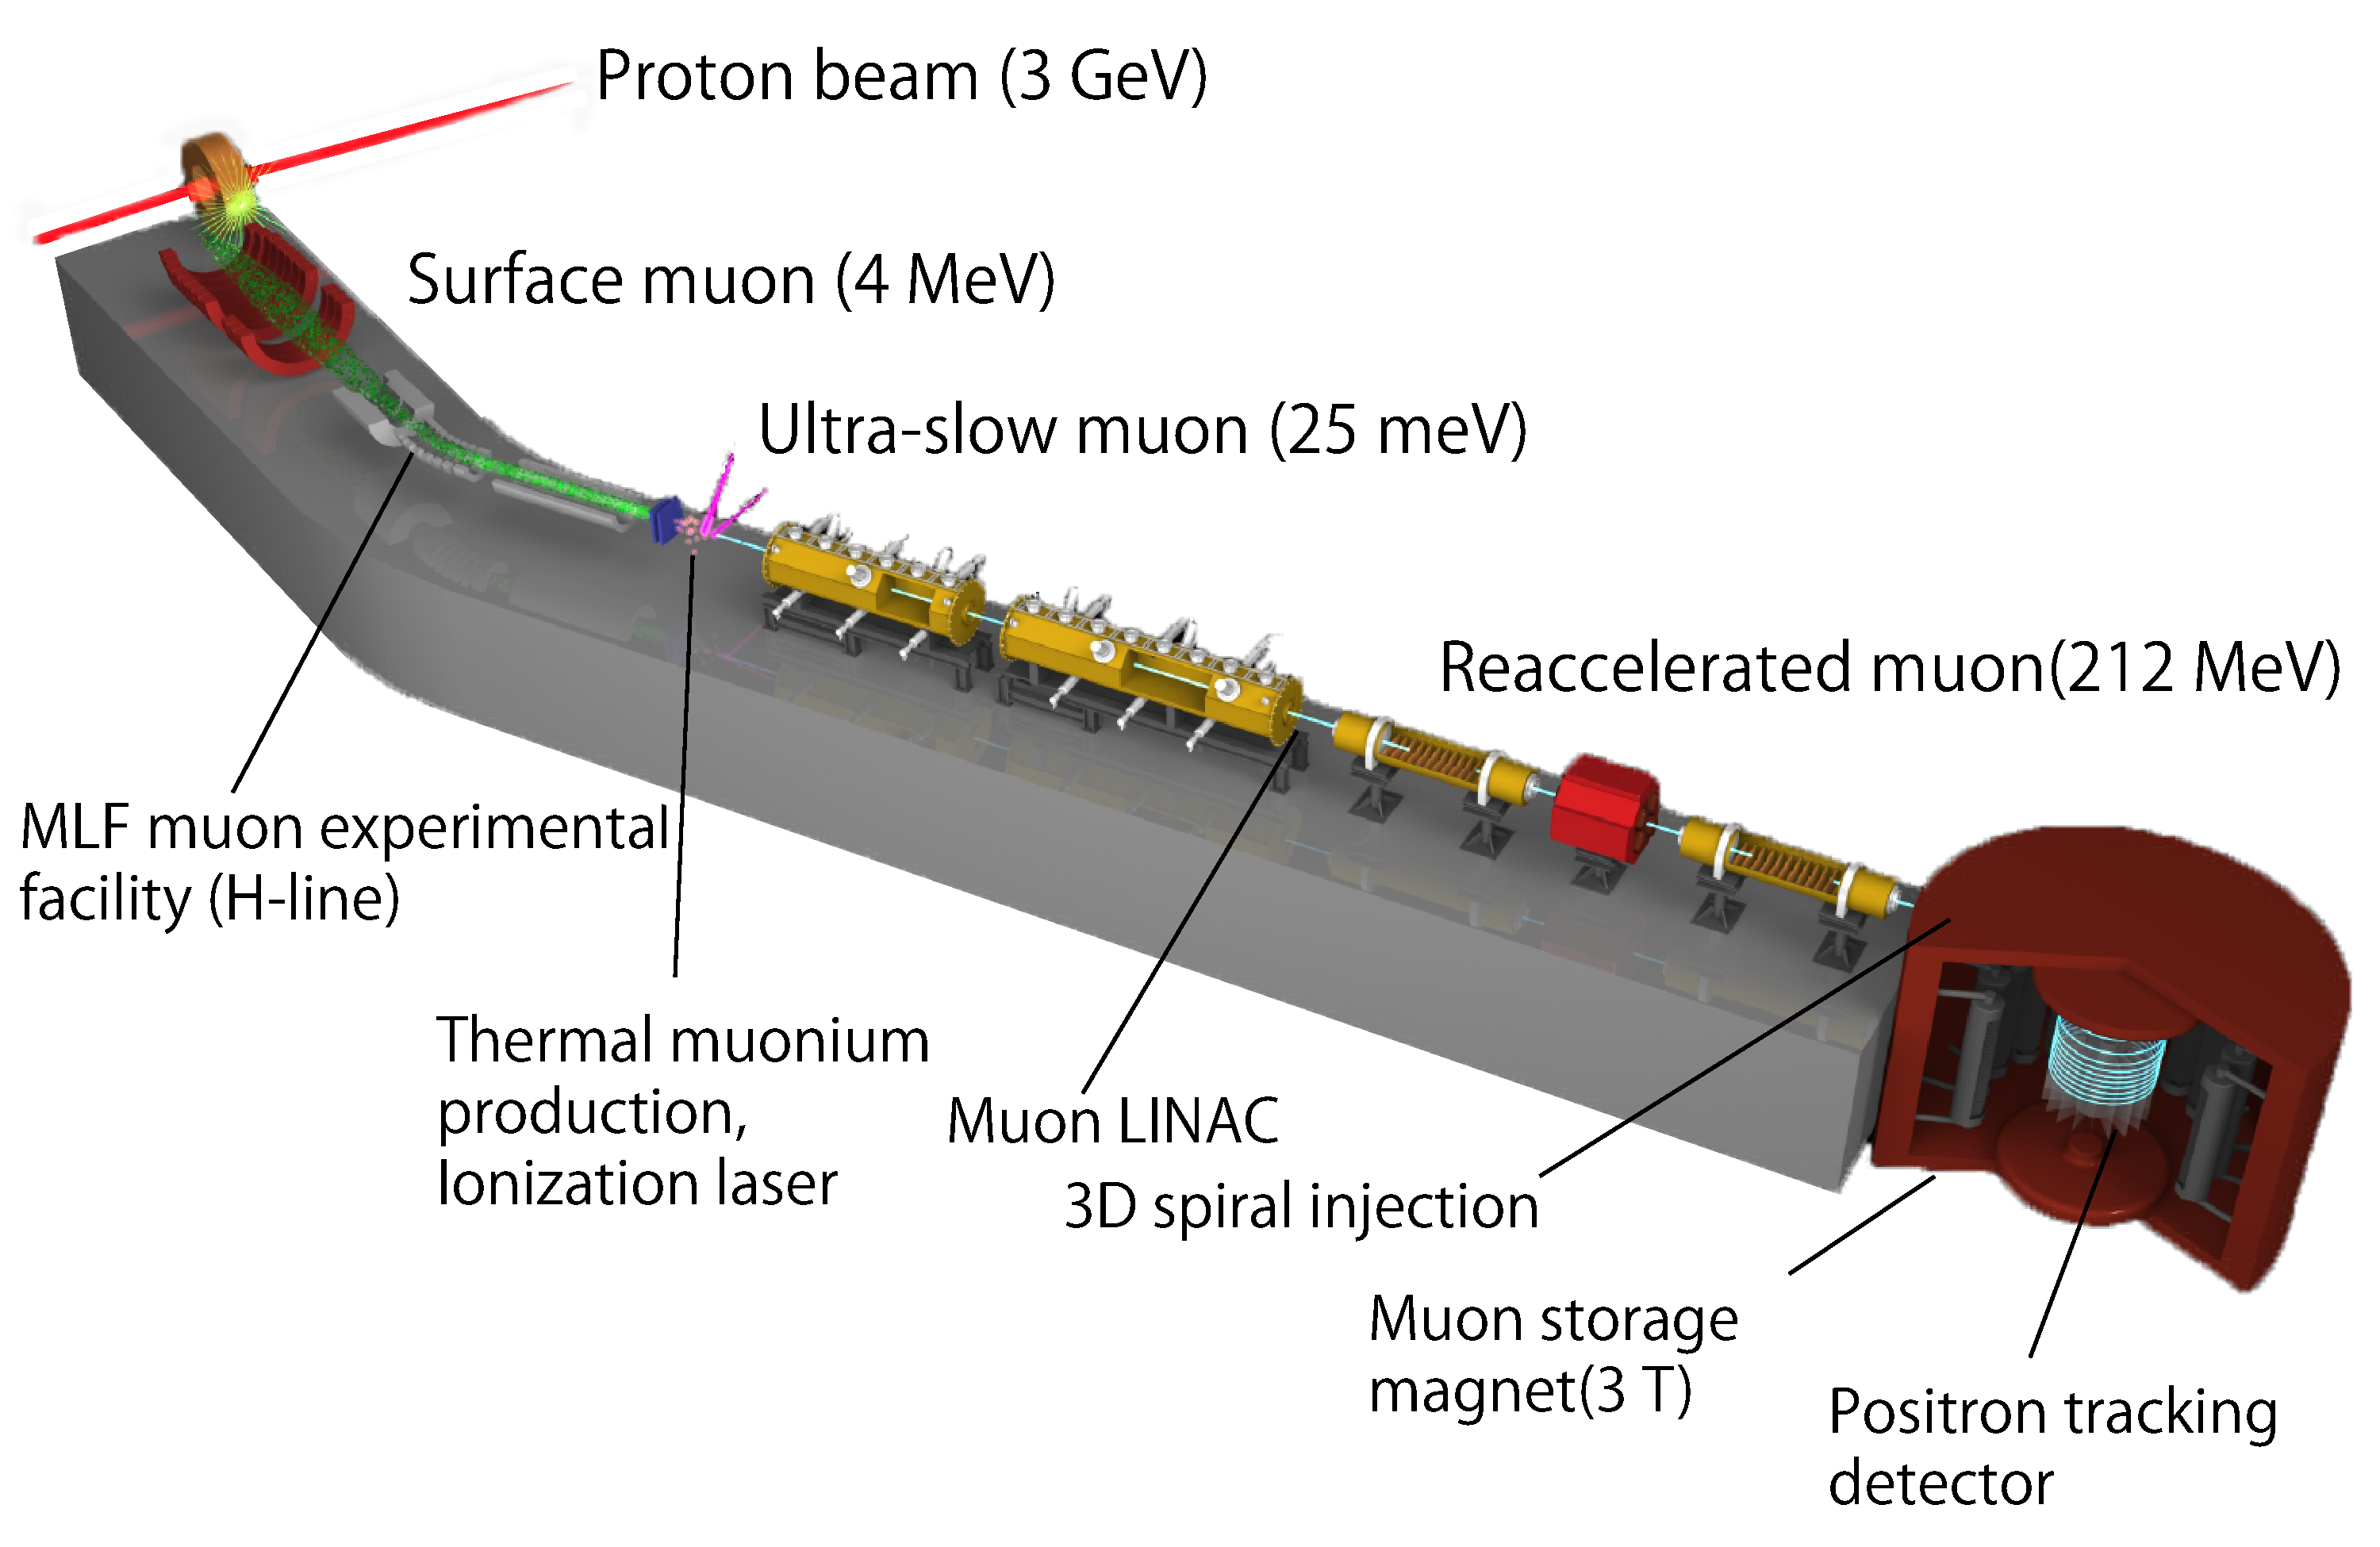
\includegraphics[width=15cm,bb=0 0 1440 936]{Fig/g-2edm_overview_en.pdf}
  \end{center}
  \caption{Schematic of the muon $g-2$/EDM experiment at J-PARC MLF~\cite{TDRsummarypaper}. }
  \label{fig:setup}
\end{figure}

The experiment will be installed at the muon facility~\cite{Higemoto:2017} in
the Materials and Life science Facility (MLF) of J-PARC.
A schematic of the experimental setup is shown in Fig.~\ref{fig:setup}. 
Experimental components and sensitivity estimations are described in the following sections.

%====================================================
\subsection{Experimental facility and surface muon beam}
A 3~GeV primary proton beam with 1~MW beam power from the Rapid Cycle Synchrotron hits 
a 2~cm thick graphite target to provide pulsed muon beams.
The proton beam has a double-pulse structure, and each pulse is 100~ns in FWHM 
with a 600~ns separation and 25~Hz repetition rate.
The experiment uses a surface muon beam.
Surface muons are 100\% polarized positive muons from pions 
stopped at and near the target surface with the consequent momentum of 29.8 MeV/$c$ and below.
There are four beamlines extracting muon beams.
The experiment will use one of those, the H-line.

The H-line is a new beamline designed 
to deliver a high intensity muon beam~\cite{Kawamura:2014hja}.
This is realized by 
adopting a large aperture solenoid magnet to capture muons from the muon production target,
wide gap bending magnets for momentum selection,
and a pair of different directional solenoid magnets for efficient beam transport.
The surface muon beam is focused onto a target to produce muonium atoms.
The final focus condition is optimized to maximize the number of muons stopping in the muonium production 
target and to minimize the leakage magnetic field at the focal point. To fullfill these 
requirements, 
%the final focusing magnets are composed of a solenoid magnet
the final focusing includes a solenoid magnet
followed by a triplet of quadrupole magnets.

The intensity of the surface muon beam at H-line is estimated 
to $10^8$ per second at the designed proton beam power of 1 MW.
The surface muon at the end of the beamline has a momentum centered at 28.2 MeV/c with 
10\% momentum bite. According to a beam transport simulation
the beam size at the focal point will be $\sigma_x=31$~mm and $\sigma_y=14$~mm.

%===============================================================
\subsection{Production of thermal muons from surface muons} 
%
The surface muon beam is converted at its final focus into a
source of room-temperature muons. The first step is to
slow and thermalize the $\mu^{+}$ in a carefully selected
material, silica aerogel \cite{Tabata:2011aa}.  In this
material, most of the muons form muonium atoms ($\mu^{+}e^{-}$, or Mu)
that diffuses as a neutral atom into a vacuum region where Mu is
ionized by laser excitation (Fig.~\ref{fig:usm}). While the thermalization, conversion
to Mu, diffusion, and ionization steps result in the loss of a significant
fraction of the original surface muon beam, the
characteristics of thermal muons after muonium ionization can be
exploited as a source for acceleration and injection into a
storage ring. A comparison of the kinematic characteristics of
surface muons, a thermal source, and accelerated muon
is summarized in Fig.~\ref{fig:usm}.

\begin{figure}[t]
\centering
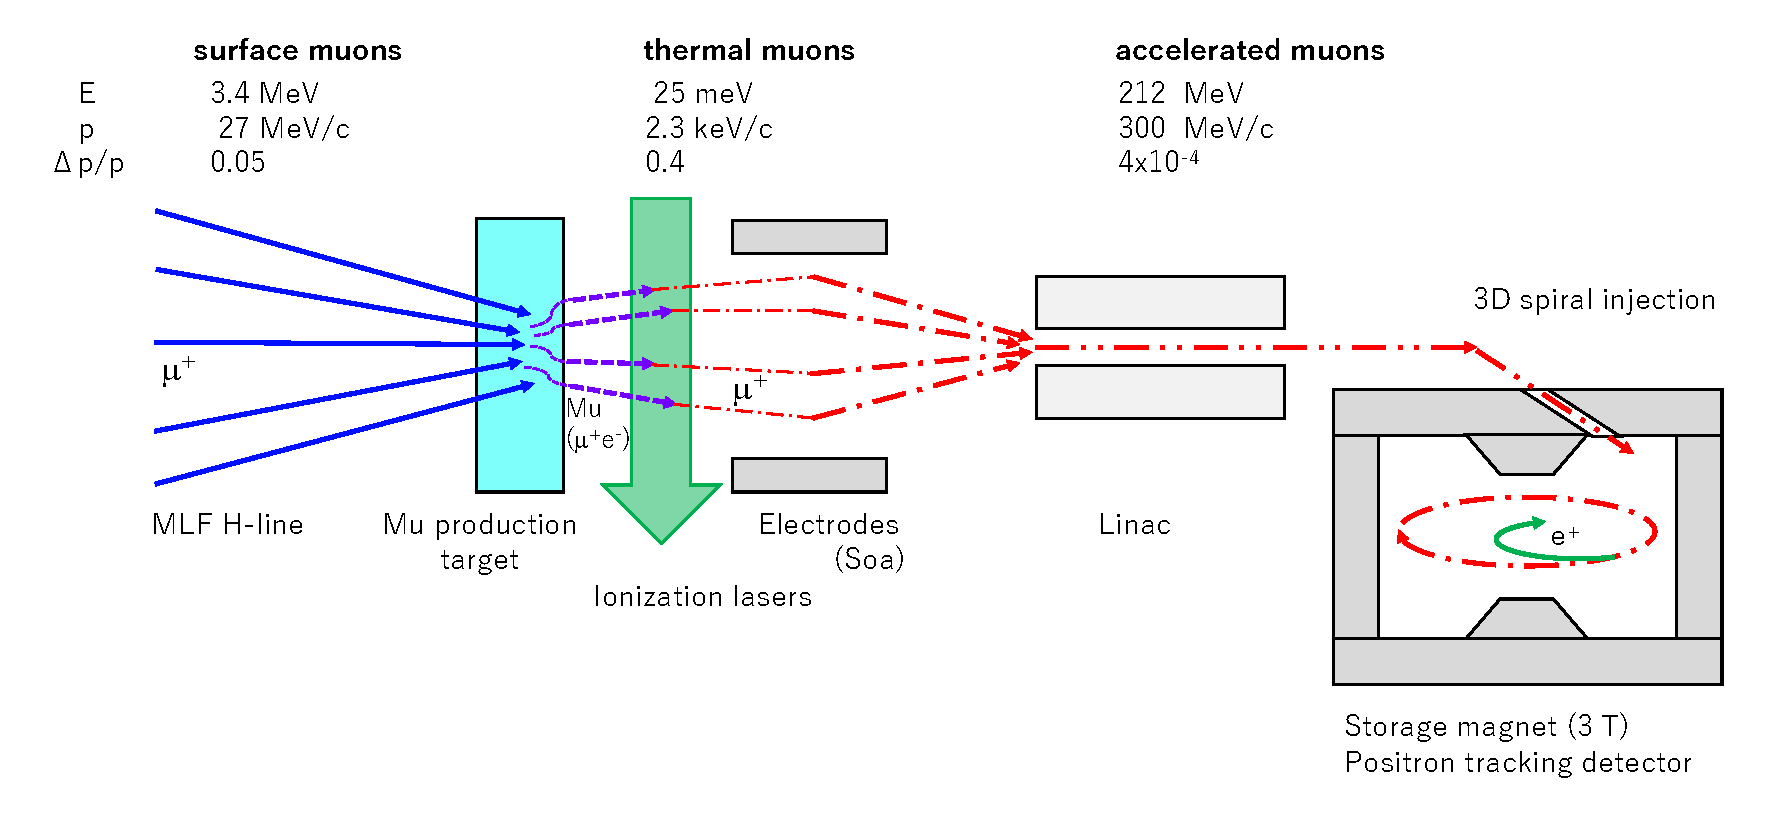
\includegraphics[width=1.0\columnwidth, bb=0 0 680 312]{Fig/muonbeam.pdf}
\caption{Scheme of the reaccelerated thermal muon beam~\cite{TDRsummarypaper}.
The surface muon beam is stopped in a silica aerogel plate at 
the downstream edge. Some of the formed muoniums diffuse to surface 
and evaporate to vacuum with thermal energy. 
Intense laser beams strip the electron from muonium 
and the muon is accelerated by a static electric field followed by 
RF acceleration. 
}
\label{fig:usm} 
\end{figure}

Silica aerogel is chosen as the muonium production target for
high Mu formation probability ($>0.5$) and low
relaxation of the polarization.
The 50\% polarization is the maximum after statistical spin
distribution among hyperfine states in the Mu atom.
In addition, the silica aerogel provides the large mobility of
Mu atoms within the aerogel structure such that they can be
emitted with a near-thermal room temperature energy distribution
from the surface of the slab into the adjacent vacuum region.

The emission of Mu from aerogel, as well as the other important
characteristics described above, has been discovered and verified by experiments
on a surface muon beam line at TRIUMF~\cite{Bakule:2013poa,Beer:2014ooa} and J-PARC.
The results showed that the
emission probability was enhanced by an order of magnitude if the
downstream aerogel surface was covered with a close-packed array of holes
produced by laser ablation to a depth of order a few mm. 
The data are consistent with the assumption of Mu diffusion 
within the aerogel slab to the surface of ablation holes 
followed by emission through the holes 
with speeds corresponding to thermal velocity near
room temperature.

The evolution of muonium into the laser irradiation region
located at 1~mm from the surface of the aerogel slab is simulated.
The laser region is defined as a volume of $40\times 40\times 5$~mm$^3$ in the transverse directions,
and the longidudinal direction, respectively.
This simulation indicates that the optimum time for the
short ionization pulse is near 1.0 $\mu$s after the
average time of arrival of the two surface muon pulses (0.6~$\mu$s apart).
The efficiency for thermal muonium production in the laser region 
is estimated as $3.8\times 10^{-3}$ per surface muon.

A high-power ionizing laser beam system is synchronized to the
periodic 25~Hz thermal Mu production at its maximum density in vacuum.
One laser at 122~nm (Ly-$\alpha$) with 80~GHz linewidth and 100~$\mu$J per pulse excites the Mu from the $1s$ atomic state
to $2p$, then a second at 355~nm with 300~mJ strips the electron. The
laser pulses are 1~ns duration. The estimated ionization efficiency of this process is 73\%.
The generation of coherent Ly-$\alpha$ light is realized by using a nonlinear conversion process 
of the two-photon resonance four-wave difference frequency mixing in Kr gas.
The feed lights are generated by a solid state laser system consisting of 
a fiber coupled distributed feedback laser diode followed by
three stages of amplification and nonlinear conversions.
Such an intense Lyman-$\alpha$ laser \cite{laser:2016} is being developed 
in collaboration with the group developing an ultra slow muon microscope, which 
is being used for the ionization of muonium at J-PARC U-line \cite{usm:2018}. 


%=========================================================
\subsection{Acceleration}

%%%%%%%%%%
%Overview
%%%%%%%%%%

The room-temperature muons created in the laser ionization of thermal muonium will be 
accelerated to a momentum of 300~MeV/$c$ (212~MeV in kinetic energy).
The muons must be accelerated in a sufficiently short time
compared with the muon life time of 2.2~$\mu$s
to suppress muon decay loss during the acceleration.
Another essential requirement for the acceleration is
the suppression of transverse emittance growth.
To satisfy these, a linac dedicated to this purpose will be used in the experiment.
Figure~\ref{fig:mulinac_config} shows the schematic configuration
of the muon linac.
In accelerating the muons, the $\beta$ increases rapidly with the
kinetic energy.
It is important to adopt adequate 
accelerating structures to obtain high acceleration efficiency,
similar to proton linacs. 
The acceleration steps are 1) electrostatic acceleration with a Soa lens,
2) radio frequency quadrupole (RFQ),
3) inter-digital H-type drift tube linac (IH-DTL),
4) disk-and-washer structure (DAW),
and 5) disk-loaded traveling wave structure (DLS).

\begin{figure}[t]
\centering
\includegraphics*[width=1.0\textwidth,bb=0 0 680 170]{Fig/muonlinac.pdf}
\caption{Schematic configuration of the muon linac~\cite{TDRsummarypaper}.}
\label{fig:mulinac_config}
\end{figure}

%%%%%%%%%%%
% Init Acc
%%%%%%%%%%%

 As the first acceleration step, thermal muons are accelerated from the ionization region
by a pair of meshed metal plates and an electro-static lens, a Soa lens~\cite{Soa}.
The ellipses in the $x$-$x^{\prime}$ and $y$-$y^{\prime}$ distributions represent
the matched ellipses of 1.0$\pi$~mm~mrad.
The lower right figure represents the time structure at the entrance
of the RFQ.
Even though the pulse width of the dissociation laser is 1~ns,
the time width at the RFQ entrance is 10~ns
owing to the spatial distribution at ionization.
Therefore, the beam from the source divides into three bunches during 
the acceeleration in the RFQ at the frequency of 324~MHz.
A spare RFQ of the J-PARC linac~\cite{kondo:hptest_rfqII:prstab2013}
will be used as a front-end accelerating
structure accelerating the muons to 0.34~keV~\cite{kondo:simulation_mu_rfq:ipac2015}.

%%%%%
% IH
%%%%% 
\newcommand{\Ez}{E_{z}}

The energy of the muon beam is boosted to 4.5~MeV with an IH-DTL.
Different from the Alvarez DTL, the IH-DTL uses the TE11 eigenmode,
and $\pi$-mode acceleration~\cite{bib:IH_blewette}. 
With this mode, the acceleration length is halved compared with
the 2$\pi$-mode acceleration. 
In addition, alternative phase focusing (APF)~\cite{bib:IH_APF1} is adopted.
Since the use of APF eliminates the need for installing quadrupoles
in the drift tubes, a higher shunt impedance per length can be achieved. 
The beam dynamics with such an IH-DTL was studied~\cite{Otani:2016swo}.
Sixteen cells are required to accelerate up to 4.5~MeV,
and the total length of the cells is 1.29~m. 
The quality factor $Q_{0}$ is calculated to be $1.03\times 10^{4}$, 
and the power dissipation is 320~kW. 
The effective shunt impedance per unit length is calculated
to be 58~$\mathrm{M\Omega/m}$,
which is competitive with those of other IH structures, taking 
our IH application to a relatively higher velocity region into account. 

%%%%%%
% DAW
%%%%%%

Following the IH-DTL, DAW structures
with a frequency of 1,296~MHz are used accelerate to 40~MeV.
The DAW is one of the coupled-cavity linacs which has large coupling 
between the cells and a high shunt impedance, especially in the middle
$\beta$ section~\cite{andreev:he_proton_linac_structures:linac1972}. 
The cell design was optimized for the velocities of 
$\beta=0.3, 0.4, 0.5,$ and $0.6$ 
by using the SIMPLEX algorithm~\cite{otani:develop_mulinac:ipac2016}.
PARMILA~\cite{parmila} was used to design
the beam dynamics of the DAW section.
The acceleration gradient is determined to be 5.6~MV/m so as to keep
the maximum electric field less than 0.9 times the Kilpatrick
limit~\cite{bib:kilpatrick}. 
The field strength of the quadrupole doublet between the modules and
the number of the cells in each module are determined
with a condition that the phase advance in one focusing period
is less than 90~degrees. 
The number of the cells in a module is set to ten, and  
the phase advance is approximately 83~degrees in the first module,
where the RF defocusing is strongest. 
The total length is 16.3~m with 15~modules.
The estimated power dissipation is 4.5~MW. 

%%%%%%
% DLS
%%%%%%

 Finally, the muons are accelerated from 40~MeV to 212~MeV by using a DLS,
which are widely used for electron linacs.
 The advantage of the DLS is its high acceleration gradient;
approximately 20~MV/m.
 An RF frequency of 1,296~MHz is adequate for the wider phase space.
The particular design feature of the DLS for
the muon acceleration, which is different from 
the general accelerating structure for the electron accelerator, 
is the variation of the disk spacing corresponding to 
the muon velocity~\cite{kondo:beamdynamics_muon_highbeta:ipac2017}.
 The DLS section consists of four accelerating structures and 
the total length is approximately 10~m.
The estimated momentum spread is 
0.04~\%(RMS).

With this design of the muon linac, these simulations show that the transmission efficiency is kept high,
and there is no significant growth of the beam emittance during the acceleration.

%===============================================================
\subsection{Beam injection and muon storage magnet}

The muon beam must be injected into the muon storage magnet and the injection system
must have minimum interference to the storage field. For reasons described later,
a new method to inject the muon beam from the top of the magnet is adopted.
After the linac, the muon beam follows a beam transport line to inject the muon 
beam at an incident vertical angle of 25~degrees. The beam transport line consists of 
two dipole magnets for bending the beam vertically, three normal quadrupole magnets
to match the vertical momentum dispersion and eight rotated quadrupole magnets
to control the phasespace to match the acceptance of injection into the magnet.

\begin{figure}[t]
%\vspace*{-0.3cm}
%\vspace*{7.0cm}
 \centerline{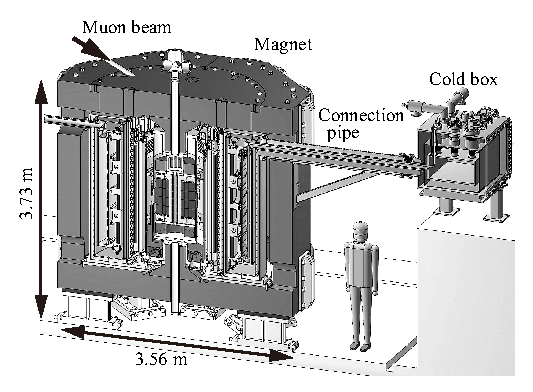
\includegraphics[width=12cm]{Fig/MagnetMechOverviewBW.eps}}
 \caption{Overview of the muon storage magnet~\cite{TDRsummarypaper}.}
\label{fig:magdesign}
%\vspace*{-0.3cm}
\end{figure}

A $3$~T MRI-type superconducting solenoid magnet will be used to complete the injection and store the muon beam.
Figure~\ref{fig:magdesign} shows an overview of the muon storage magnet~\cite{sasaki:2016}.
The muons are stored in a 3~T magnetic field with a cyclotron radius of $333$~mm.
The size of the storage magnet is about a factor of 20 smaller than the magnet for BNL/Fermilab experiments.
We take advantage of the advance in MRI magnet technology to fabricate such a small storage magnet with a highly uniform magnetic field in the muon storage region.
The magnet system has four functions: (1) provide a high uniform storage field; 
(2) provide the injection field; (3) provide the kicked field to store the muons; 
and (4) provide weak focusing for storage.

The main feature is a highly homogeneous magnetic field of $3$~T (main field) 
in the central region of the magnet, the storage region, where the muon beam is stored until its decay. 
The homogeneity of magnetic field in the storage region is directly related to the sensitivity of the $a_{\mu}$ measurement.
The integrated magnetic main field uniformity along the beam orbit in the storage region has to
be carefully controlled with a precision of $100$~ppb peak-to-peak.
The relative field distribution in the r-z plane around the storage region, averaged over the muon orbit has a variation less than $\pm 50$~ppb. 
This field uniformity is a feature of this experiment; the field variation along the muon orbit for the BNL~(E$821$) magnet was as large as $\pm$~100 ppm.

The second function is to transport the muon beam from the outside of the storage magnet to the storage region. 
This transportation region is named the injection region.
Due to the limited space of the storage magnet, the muon beam is not injected by the previous method used for CERN, BNL and Fermilab $g-2$ experiments of horizontal injection using an inflector magnet with poor ($2\sim5\%$) efficiency. 
Instead, a new $3$-D spiral injection scheme~\cite{Iinuma:2016zfu} is developed for this purpose.

A solenoid magnetic field shape is suitable for this new injection scheme. 
In the injection region, the radial component, $B_{r}$, of the magnetic field has to be carefully controlled from the top end of the magnet to the storage region for smooth injection. 
A three-dimensional view of beam trajectories from the injection region to the storage region is also shown in the right side. 
The muon beam enters from a downward with injection angle (pitch angle) of $440$~mrad. 

Open circles along the beam indicate points, which correspond to the radial field values on the left side.  
The beam momentum is deflected by the radial component of the fringe field $B_{r}$ 
as it reaches the mid plane of the solenoid magnet. Within the first three turns, the pitch angle becomes $40$~mrad.  
We design the fringe field to control beam vertical motion.
And at the same time, this fringe field requires  
appropriate vertical-horizontal coupling (so-called $X$-$Y$~coupling in the beam coordinate) to control vertical divergence, 
because of an axial symmetric shape in the fringe field. 
The $X$-$Y$~coupling of the beam phase space, controlled by the magnet staying just upstream of the solenoid, will be carefully tuned to 
minimize the vertical beam size in the storage region. 

The third function of the magnet system is to provide a vertical kick, which will guide the beam inside the storage region.
Two pairs of one-turn coils, the kicker coils at $\pm0.4$~m in height, 
generate a pulsed radial field $B_{kick}$ to apply a vertical kick to the muon beam motion. 
The vertical beam motion from the start of the kick to the end, as well as the beam motion in the storage region.

In order to keep the beam inside of the storage region within a stable orbit,
a weak focusing magnetic field~\cite{Iinuma:2016zfu,Abe:2018tmp} will be used.
The equations of the weak focusing magnetic field are 
\begin{eqnarray}
 B_r &=& -n\frac{B_{0z}}{R}z, \\
 B_z &=& B_{0z}-n\frac{B_{0z}}{R}(r-R)+ n\frac{B_{0z}}{2R^2}z^2,  
\label{eq:weak}
\end{eqnarray}
where, $B_{0z}$ (3~T) is the field strength in the $z$ direction at the center of the storage region,
$R$ (333~mm) is the average radius of the stored beam, $n$ is the field index.
The weak focusing field is the fourth function of the magnet system.

%%%%%%
%Finally, we introduce mechanical design of the magnet system briefly. 
The solenoid will be composed of 5 main coils wound with NbTi cable
and the inner radius will be 0.8~m in the present design.
%Shim coils for compensating field errors caused by the coil misalignment and so on, are installed
%on the outside of the main coils.
An iron yoke is used to suppress a magnetic flux leakage.
The magnet has pole tips at the both ends of the solenoid coil to form the magnetic flux, with an entrance hole for injection.

The main coils will be operated with a persistent current mode with a superconducting switch.
%in order to eliminate a fluctuation of the magnetic field due to an instability of current source.
The time constant of current decay is generally expected to be less than 10 ppb/hour.
This field decay will be constantly monitored by the NMR probes during the measurement.

The weak focusing magnetic field is generated by dedicated coils, the weak focus coils, consisting
 of 8 ring coils wound with NbTi cable which are aligned in the axial direction of the magnet.
All ring coils are connected in series electrically and driven by a single power supply.

The magnetic field is shimmed by passive and active shimming systems.
The former uses iron pieces,
which are attached on support cylinders installed inside the magnet bore through holes in the iron poles in air.
The magnetic field distribution is adjusted by changing the alignment pattern of iron pieces.
Active shimming is done using a superconducting shim coils wound with NbTi cable.
They are mainly used to compensate the error field changing with time in the storage region,
and the residual error (expected to be small) after the magnetic field shimming by iron pieces.
The shim coils consist of several saddle coils which have a four fold symmetry.
Each coil is connected to independent power supply to control each current.

The main coils, the weak focus coils, and the shim coils are immersed in liquid helium to ensure good temperature stability.
%The temperature could be controlled with a precise pressure control system of the helium vessel.
The helium is re-condensed by cryocoolers for long-term, stable and cost-effective operation.
Four cryocoolers and a heat exchanger for the helium re-condensation will be installed in a cold box,
 placed apart from the magnet cryostat.
A connection pipe between the cold box and the magnet cryostat has a bellows connection,
which is a soft connection in terms of mechanical structure, so that
the vibration of cryocoolers will not be directly transferred to the magnet.

The magnetic field is measured by a system with the NMR (nuclear magnetic resonance) method.
To obtain the average magnetic field $\omega_{p}$ experienced by the muon beam,
the magnetic field is measured along the muon storage orbit (integrated) with a precision below 100 ppb level
in the main field of 3~T where local field homogeneity is 1,000 ppb level.
The NMR is the only solution with this precision.

A continuous wave type (CW) NMR will be used in this experiment. 
The resonant absorption signals of protons in water samples is observed
by using a fixed frequency source and a small sweeping magnetic field.
The NMR probe will have a size of about 5 -- 10~mm in diameter.
The magnetic field in the storage region will be mapped by scanning the probe with moving stages.
The stages are driven by ultrasonic motors, which can work in the strong magnetic field.
The ultrasonic motors have encoders so that the position of NMR probe is controlled
with a precision of below 0.1~mm.

%===============================================================
\subsection{Positron Detector}\label{sec:detector}

The positron detector is installed inside of the storage magnet
and measures positron tracks from decay of stored muon beam.
A muon with the momentum of 300~MeV/$c$ circulates with a radius
of 333~mm and decays to a positron, a neutrino and an anti-neutrino
with the life time of 6.6~$\mu$s. The cyclotron period is 7.4~ns.
Since the anomalous precession period is 2.2~$\mu$s, muons circulate
the ring about 300 times on average during one revolution of muon spin.
The goals of the detector are to measure $\omega_{a}$
and the up-down asymmetry of positron direction due to EDM.

%Since the muon decay breaks the parity, high-energy positrons in their decay
Since the muon decay breaks parity, high-energy decay positrons tend to be emitted
in the direction of muon spin~\cite{Michel}. By measuring high energy positrons
selectively, positrons emitted forward can be selected and
the time variation of muon spin with respect to the muon momentum direction
can be measured. The sensitivity becomes maximum when positrons
with momentum above 200~MeV/$c$ are counted.

Positrons emitted within the 3~T magnetic field move in a spiral orbit.
This trajectory is detected by radially arranged silicon strip sensors.
Geometrical coverage of the detector is ***--290~mm in radial direction and within $\pm$400~mm
in height. Layout of the detector is shown in 
Fig.~\ref{fig:Detector_overview}. 

\begin{figure}[t]
  \begin{center}
    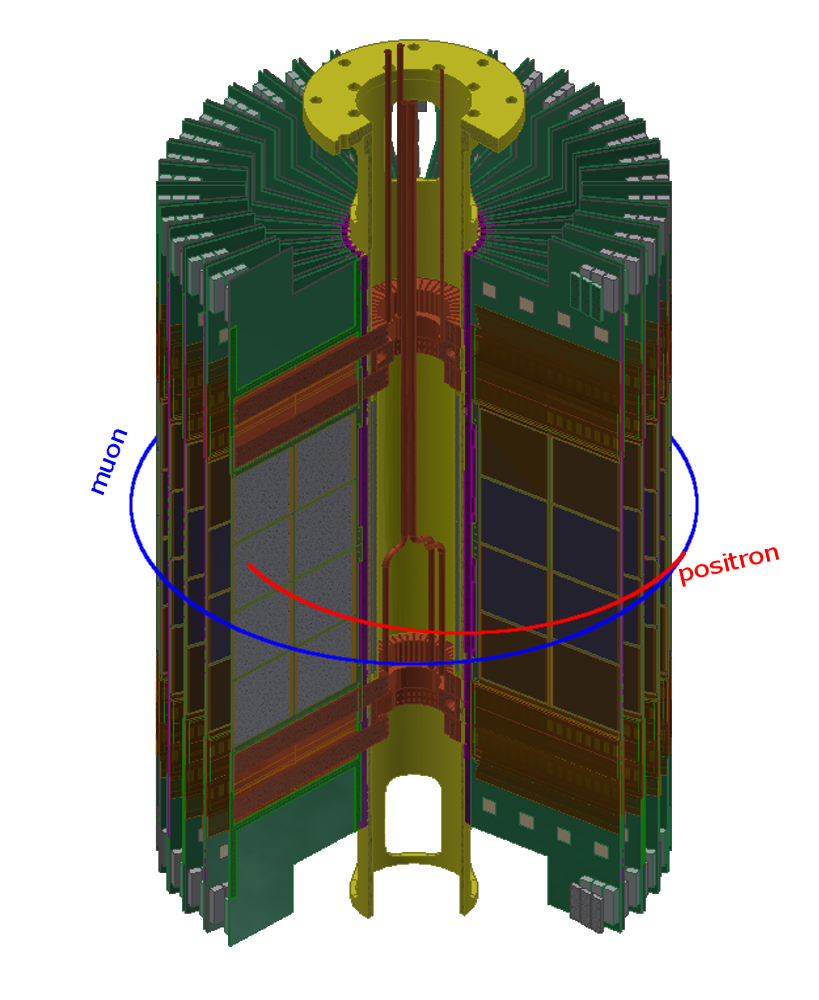
\includegraphics[width=0.4\textwidth, bb=0 0 393 511]{Fig/Detector_cutview.png}
    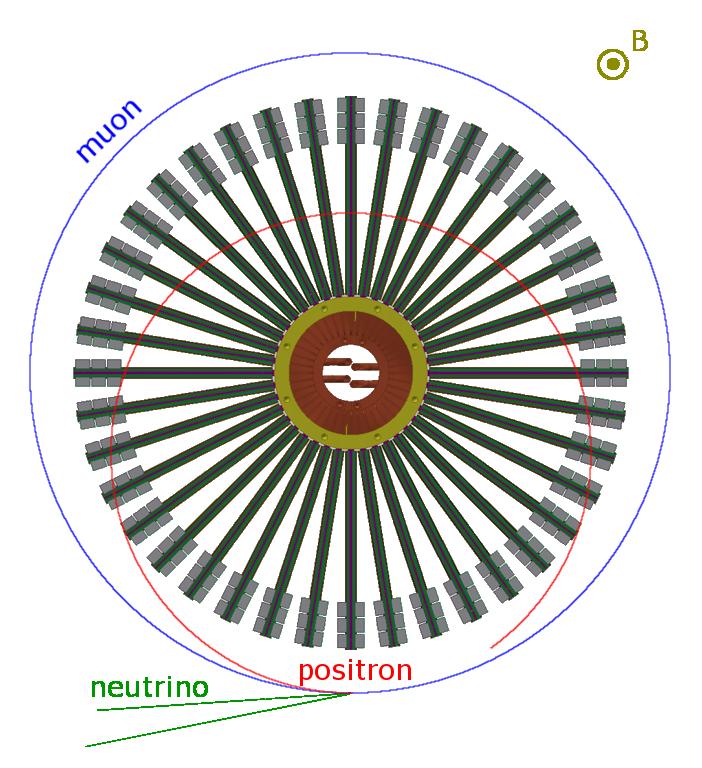
\includegraphics[width=0.4\textwidth, bb=0 0 337 369]{Fig/Detector_topview.png}
    \caption{Perspective view (left) and top view (right) of the positron detector~\cite{TDRsummarypaper}.}
    \label{fig:Detector_overview}
  \end{center}
\end{figure}

Muon beam spill rate is 25~Hz and the number of muons per spill is about $10^4$.
The measurement will be performed in the period of 33~$\mu$s, which is
 five times larger than the muon life time. The rate of positrons
changes by a factor of 160 from the beginning to the end of the measurement.
Thus, the detector is required to be stable against the change of positron rate;
otherwise, the measured $\omega_a$ would be biased.

The detector consists of 40 radial modules called vanes.
Each vane consists of 16 sensors.
Sensors are made by single-sided p-on-n technology~\cite{sensor}.
The active area of a sensor is 97.28 mm $\times$ 97.28 mm with
a thickness of 0.32~mm.
A sensor has two blocks of 512 strips and the number of strips
with 190~$\mu$m pitch. Therefore a vane has 16,384 strips, with 655k total strips for the detector.

The data from the silicon strip sensors are read out by front-end
boards on the detector with a 5~ns time stamp, followed by readout boards with 
VME interface,
then collected by the PC farm through a Gibabit Ethernet switch.
%The data size of one hit is 8 bytes when the leading and trailing edges are separately recorded.
The data acquisition system based on DAQ-Middleware~\cite{DAQ-Middleware} is used.
Estimated size of data from the whole detector is 360~MB/s (or 14.4~MB/spill).

One readout ASIC has 128 channels for analog block and digital block.
Dynamic range of input charge is required to be greater than
4 minimum ionizing particle (MIP) equivalent with linearity.
Equivalent noise charge is required to be less than 
1600~e$^{-}$ with the input capacitance of 30~pF, which
corresponds to the signal-to-noise ratio greater than 15
for a 1~MIP signal. Pulse width at 1~MIP charge is required to
be less than 50~ns and the time-walk between 0.5~MIP and 3~MIP
is required to be less than 5~ns to constrain a timing shift effect
due to pileup hits.

The system clock is provided by the GPS-synchronized Rb frequency
standard~\cite{freqtime}, and it is distributed with real time control signals
to the readout boards and the front-end board through the timing
control/monitor board. Long term stability of the system clock
frequency is confirmed better than $10^{-11}$.

The stringent requirement on the detector alignment comes
from the EDM measurement~\cite{EDM_requirement}. Alignment accuracies of vanes
with respect to the magnetic field direction
are required to be better than 10~$\mu$rad for skew, that is an
angle around an axis normal to the vane. 
In order to ensure the required accuracies, alignment changes for the
vanes are detected and monitored during operation using an absolute
distance interferometer system.

At the beginning of spill, about 30 positrons are produced from muon decay in 5~ns which is one time window of the data taking.
The maximum hit rate per silicon sensor strip is $7 \times 10^{-3}$ per time stamp.
To find positron tracks in such a condition,
a positron track candidate is searched from hits on the detector
using the property that high momentum positron tracks leave
nearly straight lines in the $\phi$-$z$ plane, 
where the $z$-axis is the center axis of the detector along the direction of magnetic field and $\phi$ is the angle around $z$-axis.
In the $\phi$-$z$ plane, (bottom right) straight lines used as seeds for track finding are shown.
Hough transformation~\cite{HoughTransform,UseHough} is used
to find straight lines in the plane and hits on a straight line are used as the seed. 
Track momentum is obtained
by track fitting with a Kalman filter~\cite{KalmanFilter}.
With this algorithm, track reconstruction efficiency
greater than 90\% is achieved in the positron energy range of
200~MeV$<E<$275~MeV even at the highest positron rate.

The muon decay position is
determined by the closest point of approach between the reconstructed positron
trajectory and the muon beam orbit.
The muon decay time at the decay position is measured by extrapolating the time of hits in reconstructed
positron tracks. 
One way to estimate decay time is to use the average time of reconstructed 
track hits.
An other approach way is to use the transition timing of hits with the 5~ns time stamp.
The latter method has better timing resolution than the former but
it is applicable only when the transition occurs within a track.
Two definitions of decay time can be cross-checked with each other.

%===============================================================
\subsection{Estimation of number of reconstructed positron}\label{sec:Intensity} 
Efficiencies of steps from the surface muon production to the detection of positrons are studied 
by a chain of simulations.
The simulations include the surface muon production,
thermal muon production, reacceleration, injection to the muon storage
magnet, muon beam dynamics in storage, and ended by the detection of the positron.
The simulation of surface muon production~\cite{otani:simulation_usm_production:ipac2018}
and thermal muon production are optimized by the experimental data
on surface muon yield at the existing beamline and measurements of muonium space-time distribution~\cite{Beer:2014ooa},
respectively.
Total efficiency is $1.4 \times 10^{-5}$ per initial muon at production.
At the proton beam power of 1~MW, the expected number of positrons is $5.7 \times 10^{11}$ for $2 \times 10^7$ seconds data taking.

\subsection{Extraction of $a_{\mu}$ and EDM}\label{sec:Sensitivities} 

The $\omega_a$ and $\eta$ are obtained from the muon decay time distribution.
The muon decay time is reconstructed from the positron track as described in Sec.~\ref{sec:detector}.
A simulated time spectrum for detected positrons in the energy range 
between 200~MeV and 275~MeV is shown in Fig.~\ref{fig:Wiggle}~(left).
The anomalous precession frequency $\omega_a$ is extracted by fitting to the data. 
Alternatively, one can make a ratio of 
data taken with different initial spin orientations.
This will be useful to study early-to-late changes in the detector performance.

\begin{figure}[t]
  \centering
    \begin{tabular}{c}

      \begin{minipage}{0.5\hsize}
        \centering
        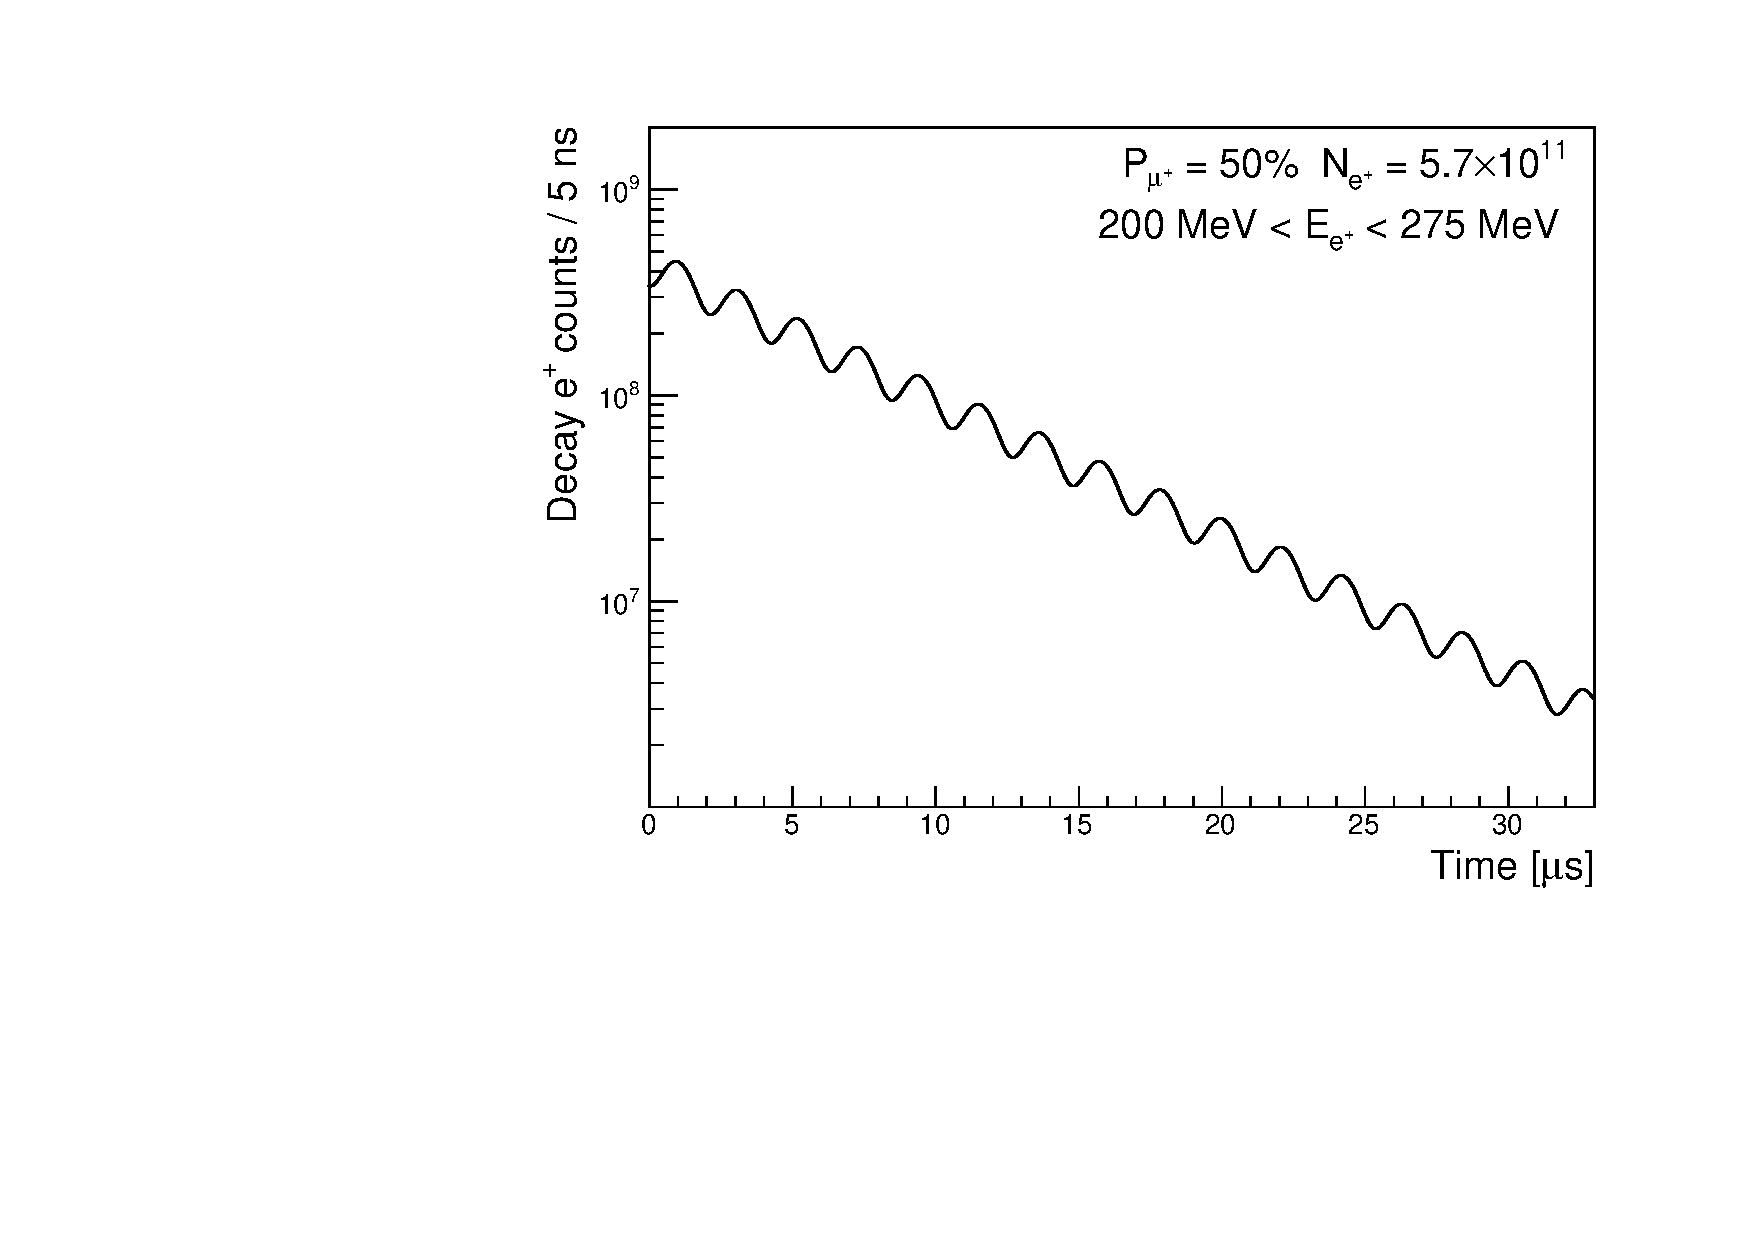
\includegraphics[width=0.7\linewidth, angle=270, bb=20 255 428 822]{Fig/WigglePlot.pdf}
      \end{minipage}

      \begin{minipage}{0.5\hsize}
        \centering
        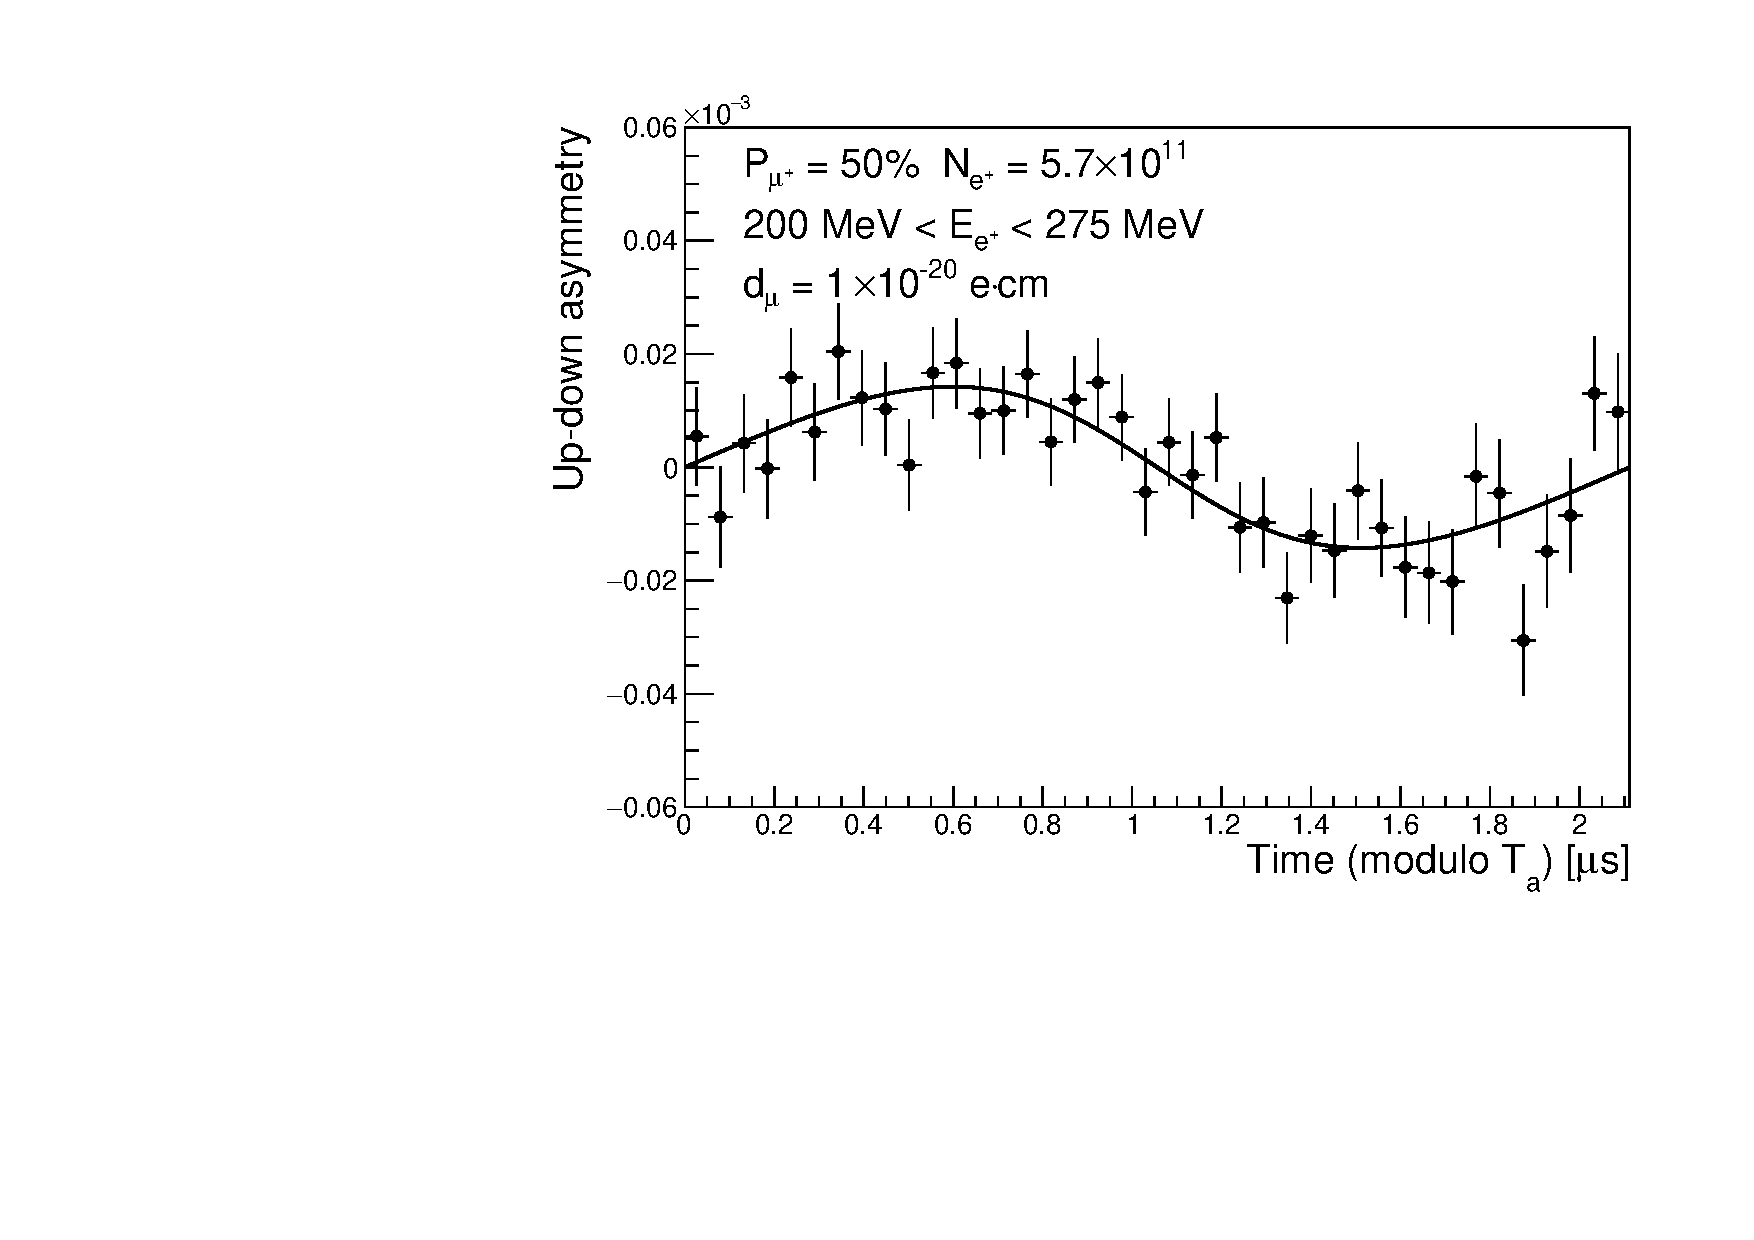
\includegraphics[width=0.7\linewidth, angle=270, bb=20 255 428 822]{Fig/EDMModuloPlot_20_40.pdf}
      \end{minipage}
    \end{tabular}

    \caption{Simulated time distribution of reconstructed positron (left) 
      and the up-down asymmery as a function of time modulo of the $g-2$ period (right).
      Solid curve is the fit to data~\cite{TDRsummarypaper}.}
    \label{fig:Wiggle}
\end{figure}

The $\omega_p$, average magnetic field seen by the muons in the storage ring, is 
measured by independent measurements of the magnetic field map in the storage ring provided from the proton
NMR data and the muon beam distribution deduced from tracing back the positron track to the muon beam.
A blind analysis will be done as was done by the previous BNL expriment, separating the results for 
magnetic field and sipin precession until all systematic uncertainties are finalized.

Once the $\omega_a$ and $\omega_p$ are extracted from the experimental
data, $a_\mu$ is obtained from Eq.~\ref{eq:amu}.
Table~\ref{tab:sensitivity} summarizes statistics and uncertainties for $2 \times 10^7$ seconds of data taking.
The estimated statistical uncertainties on $\omega_a$ and $\omega_p$ are 450~ppb and 100~ppb,
respectively. Thus, the statistical uncertainty of $a_{\mu}$ would be 460~ppb.

Systematic uncertainties on $\omega_a$ are estimated as follows.
A timing shift due to pile up of hits in the tracking detector is estimated as less than 36~ppb
in the detector simulation by taking into account time responses of readout electronics.
A correction for pitch angle is not necessary in the case of the muon storage 
in the perfect weak magnetic focusing field~\cite{Semertzidis:2016kte}. 
A difference in the actual field distribution 
from the perfect case leads to a systematic uncertainty of 13~ppb which is estimated from a precision spin-tracking simulation
of the muon beam storage.
Residual electric field modifies $\omega_a$ through the $\beta \times E$ term. 
With 1~mV/cm monitoring resolution for an E-field, the error on $\omega_a$ is 10~ppb. 
Other effects, such as delayed high-energy positrons and differential decay, are 
of the order 1~ppb.
 In the $\omega_p$ measurement, absolute calibration of the standard probe has an uncertainty of 25 ppb.
Positioning resolution of the field mapping probe at the calibration point and the muon storage
region leads to 20~ppb and 45~ppb uncertainties, respectively.
Other effects, such as field decay and eddy current from kicker are less than 10~ppb.
In summary, we estimate that the combined systematic uncertainties on $a_{\mu}$ is less than 70~ppb.

\begin{table}[t]
  \caption{Summary of statistics and uncertainties}
  \label{tab:sensitivity}
  \begin{center}
%  \begin{small}
  \begin{tabular}{|p{0.5\textwidth}|c|c}
  \hline
          & Estimation \\
    \hline
    \hline
%    Running time [s] & $2\times 10^{7}$ \\
%    Muon beam polarization & 0.5 \\ 
%    Average muon rate in the storage magnet [s$^{-1}$] & $2.6\times 10^{5}$ \\
    Total number of muons in the storage magnet & $5.2 \times 10^{12}$ \\
%    Energy range of $e^{+}$ [MeV] & [200,275] \\
%    Acceptance of the $e^{+}$ & 0.121 \\
%    Track reconstruction efficiency & 0.9 \\
    Total number of positrons &  $0.57\times 10^{12}$ \\
    Effective analyzing power &  0.42 \\
    \hline
    Statistical uncertainty on $\omega_{a}$ [ppb]  &  450 \\
    Statistical uncertainty on $\omega_{p}$ [ppb]  &  100 \\
    \hline
    Uuncertainties on $a_{\mu}$ [ppb]  & 460 (stat.) \\ 
                                                            & $<70$ (syst.) \\
    \hline
    Uncertainties on EDM [$10^{-21}~e\cdot$cm]  & 1.4 (stat.) \\
                                                                              & 0.36 (syst.) \\
    \hline
  \end{tabular}
%  \end{small}
  \end{center}
\end{table}

 A muon EDM will produce muon spin precession out of
the horizontal plane that is defined by the ideal muon orbit.
This can be seen from Eq.~\ref{eq:omega_tot}
where the second term is the EDM term that is perpendicular
to the $a_\mu$ term. Due to the fact that the EDM term generates
vertical motion of the spin, one can extract the EDM term
from the oscillation of the up and down asymmetry $\mathcal{A}_{UD}(t)$ in
number of positrons detected,
\begin{eqnarray}
\mathcal{A}_{UD}(t) = 
\frac{N^{up}(t) - N^{down}(t)}{N^{up}(t) + N^{down}(t)} =
\frac{PA_{EDM} \sin{(\omega_{tot}t+\phi)}}{1+ P A \cos{(\omega_{tot}t+\phi)}},
\end{eqnarray}
where $P$ and $A$ are the polarization of the muon and an effective analyzing power of muon decay, respectively. $A_{EDM}$ is an effective analyzing power associated with the EDM.
A simulated up-down asymmetry in the case of $d_{\mu}=1\times 10^{-20}~e\cdot\mbox{cm}$ 
is shown in Fig.~\ref{fig:Wiggle}~(right).
The estimated statistical sensitivity for EDM is $1.5\times 10^{-21}~e\cdot\mbox{cm}$ (See Table~\ref{tab:sensitivity}).

A major source of systematic uncertainties on EDM is detector misalignment with respect to
the plane of the muon storage. The alignment resolution is estimated as 
$0.36\times 10^{-21}~e\cdot\mbox{cm}$ from the resolution 
of the alignment monitor system made with an optical frequency comb technology.
Effects of axial electric field and radial magnetic field~\cite{Silenko:2017vvd}
are both less than $10^{-24}~e\cdot\mbox{cm}$, thus negligibly small.

%===============================================================
\subsection{Summary and prospects}\label{sec:Summary} 

%In summary, 
A new method of measuring $a_{\mu}$ and EDM of the muon is described.
The experiment utilizes a low-emittance muon beam prepared by 
reaccelerating thermal-energy muons created from laser-resonant 
ionization of muonium atoms. The low emittance muon beam allows use of a very
weak magnetic focusing and the selected low muon momentum (300~MeV/$c$) leads to use of a compact magnetic storage ring, 
instead of strong electric focusing at the magic momentum (3~GeV/$c$) used by previous and ongoing $g-2$ experiments.
A novel three dimensional spiral injection method with a pulsed magnetic kick
is adopted to store the muon beam in the storage ring efficiently.
The experiment reconstructs positron tracks from muons decay during their storage 
with a tracking detector consisted of silicon-strip sensors.

This experiment intends to reach statistical
uncertainties for $a_{\mu}$ of 460~ppb and for muon EDM of
$1.5\times 10^{-21}~e\cdot\mbox{cm}$, for an acquisition time
of $2 \times 10^7$ seconds. The statistical precision is comparable to
that of the BNL experiment. The EDM sensitivity is about two orders of magnitude
smaller than the BNL limits.
{Present estimates of systematic uncertainties on $a_{\mu}$ and EDM are
factor of seven and four smaller than the statistical uncertainties, respectively.
This experiment will test the 3~$\sigma$ deviation on $g-2$ reported by
the BNL experiment with significantly different and improved systematic uncertainties 
and search for new sources of T-violation in the muon with unprecedented sensitivity.


%\section{Muonium hyperfine splitting measurement at J-PARC}
\section{Muonium hyperfine structure measurement}

Muonium is a hydrogen-like atom made of a positive muon and
an electron.  High precision measurements of the muonium ground
state hyperfine structure (HFS) is one of the most sensitive
test for bound state quantum electrodynamics (QED), and for
determining precisely fundamental constants of the muon magnetic
moment and hence its mass.  Indeed, hydrogen HFS is the most
precisely measured value with a precision 0.2 ppt \cite{Essen-1973},
but the theoretical value is presently limited at
0.6 ppm \cite{Eides:1012805} due to the proton internal structure.
In addition, the hyperfine structure of positronium, which
is a bound state of a positron and an electron, is limited
experimentally by its mean lifetime (i.e. 140 ns for
ortho-positronium) with an accuracy of only
3.3 ppm \cite{Ritter-etal, Mills, Ishida-etal-PLB734-338-2014},
while its theoretical value is calculated at
a level of 1.1 ppm \cite{Baker-etal-PRL.112.120407} with
uncertainties from unknown nonlogarithmic
higher-order terms.  However, lifetime of the muonium (2.2 $\mu$s)
is long enough to precisely measure hyperfine structure, and
due to its constituents have an no internal structure (pure
leptonic system), hyperfine structure can be accurately calculated.
The previous muonium HFS measurement at zero field \cite{Casperson-etal}
reached a precision of 310 ppb, while the one at high 
field \cite{Liu:1999iz} achieved
12 ppb, both performed at LAMPF and with experimental uncertainties
mostly dominated by statistical errors.  The current theoretical
value of muonium HFS is 61 ppb \cite{CODATA}, but it is reported
that effort to reach 10 ppb level is in progress.

In addition to test QED, it should be noted that the experimental
values of the muon magnetic moment and mass are currently determined
by the previous muonium HFS experiment at high
field \cite{Liu:1999iz}.  The
magnetic moment ratio between muon and proton is of the utmost
importance in the determination of the muon anomalous magnetic
moment, also called muon $g-2$, and being regarded as a keystone
at unravelling the physics of the standard model and 
beyond \cite{Otani-JPARCSympo-2015}.
Furthermore, precision microwave spectroscopy of muonium can
also contribute to many new physics such as testing CPT and
Lorentz invariance incorporated in extensions to the standard
model \cite{Hughes-etal-inBook, KosteleckyVargas-PRD92.056002},
disentangling the proton radius puzzle \cite{Pohl-etal-nature,
Brodsky-etal-PRL94.022001},
searching for exotic particle \cite{Karshenboim-PRL104.220406,
KarshenboimFlambaum-PRA84-2011}, and even probing for
long-range neutrino-mediated forces \cite{Stadnik}.

The MuSEUM collaboration is now planning new and complementary
measurements of the muonium HFS both at zero field and at a high
magnetic field of 1.7 T.  Our goal is to improve the precision
of these measurements by one order of magnitude.  The new
high-intensity surface muon beamline, H-Line, that will soon be
available at J-PARC MUSE \cite{Higemoto:2017}, will provide
an opportunity to achieve that goal.

However, as we improve the statistics, understanding and suppressing
systematic uncertainty become essential.  Developments were performed
and tools have been created to suppress uncertainties associated
with the magnetic field inhomogeneity, muon stopping distribution,
microwave power fluctuation and gas density extrapolation.  An
overview of the different aspects of these new precise muonium
HFS measurements, the current status of the preparation for
high-field measurements, and the latest measurements at zero
field are presented.


The muonium hyperfine is measured by the spectroscopy of the
spin states.  The Hamiltonian of the ground state muonium is
expressed as
%
\begin{align}
 H  =    h \nu_{\text{HFS}} \mathbf{s}_\mu \cdot \mathbf{s}_e
      - \mu_\mu g'_\mu \mathbf{s}_\mu \cdot \mathbf{H} 
      + \mu_e g'_e \mathbf{s}_e \cdot \mathbf{H} 
\end{align}
%
where $\nu_{\text{HFS}}$ is the muonium hyperfine structure,
$\mu_\mu$ ($\mu_e$) is the magnetic moment, $g'_\mu$ ($g'_e$)
is the bound $g$-factor of muon and electron in the muonium,
and $\mathbf{s}_\mu$ ($\mathbf{s}_e$) is the spin of the muon
(electron).  The muonium hyperfine structure is measured by
the measurement at $\mathbf{H}=0$ by measuring the energy level
between the spin singlet and triplet.  When $\mathbf{H}$
is non-zero, the spin triplet split to three sublevels, which
is called the Zeeman effect.  Figure \ref{fig:BreitRabi} shows
the Breit Rabi diagram of the muonium 1S$_{1/2}$ state.

\begin{figure}[th]
 \centering
 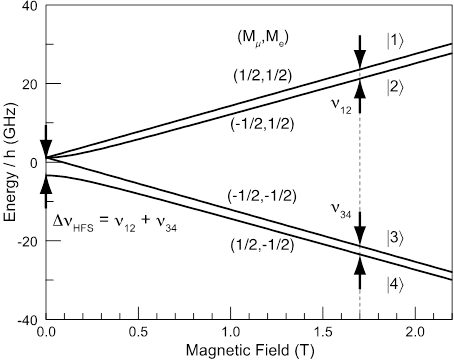
\includegraphics[width=0.5\textwidth, bb= 0 0 227 181]
                 {./Fig/MuHFS-BreitRabi.png}
\caption{\label{fig:BreitRabi}
Breit-Rabi energy level diagram for muonium atom under magnetic field.}
\end{figure}

In the MuHFS measurement with high magnetic field,magnetic
moment ratio of muon and proton can be derived from the
transition frequencies between the Zeeman sublevels $\nu_{12}$
and $\nu_{34}$ which are expressed as 
%
\begin{align}
\nu_{12}&= \frac{\mu_\mu g'_\mu H}{h}
           + \frac{\nu_{\text{HFS}}}{2}
             \left[ (1+x) - \sqrt{1+x^2} \right]~,\\
\nu_{34}&= \frac{\mu_\mu g'_\mu H}{h}
           + \frac{\nu_{\text{HFS}}}{2}
             \left[ (1+x) + \sqrt{1+x^2} \right]~,
\end{align}
%
where $x=\frac{(g'_e \mu_e + g'_\mu \mu_\mu)H}{h\nu_{\text{HFS}}}$.
The magnetic field $H$ can be measured with the nuclear magnetic
resonance (NMR) precession frequency of free proton $\mu_p$
as $h\nu_p = 2\mu_p H$.  Therefore, the muonium hyperfine
structure can be measured by $\nu_{\text{HFS}}=\nu_{12}+\nu_{34}$
and also the muon to proton magnetic moment ratio is derived
by $\nu_{12}, \nu_{34}$ and $\nu_p$.  This value is measured
at LAMPF with 120 ppb precision as $\mu_\mu/\mu_p =
3.183 \, 345  \, 24(37)$.  This measurement is also used to
determine the values of the muon to electron mass ratio.
%
\begin{align}
\frac{m_\mu}{m_e}
=
\left( \frac{g_\mu}{g_e} \right)
\left( \frac{\mu_\mu}{\mu_p} \right)^{-1}
\left( \frac{\mu_e}{\mu_p} \right) ~.
\end{align}
%
As the major uncertainty of this formula is caused by
$\mu_\mu/\mu_p$, therefore the precision of the muon-electron
mass ratio is determined as $m_\mu/m_e= 206.768 \, 276(24)$ (120ppb).
$m_\mu/m_e$ is also measured in other methods.for example, the
muonium 1S-2S interval measurement by the Doppler-free two-photon
laser spectroscopy, $m_\mu/m_e$ was extracted as $206.768 \, 38(17)$
\cite{Meyer-etal-PRL84.1136}.  By combining other experimental
results and comparing to the theoretical prediction, we can
have a stringent test of the bound state QED also with $m_\mu/m_e$.


\begin{figure}[th]
 \centering
 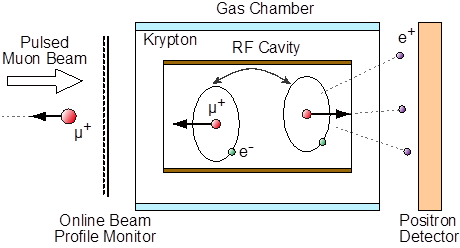
\includegraphics[width=0.7\textwidth, bb=0 0 230 124]
                 {./Fig/MuHFS-MuSEUM-setup.png}
\caption{\label{fig:MuSEUM-setup}
Schematic view of the experimental setup.  This apparatus is
either enclosed in a magnetic shield box for zero-field
measurements, or inserted in a large superconducting solenoid
magnet for high-field measurements.}
\end{figure}

The schematic view of the experimental setup is shown in
Fig.~\ref{fig:MuSEUM-setup}, and the experimental procedure
can be summarized as follows: (1) muonium formation, (2) RF
spin flip, and (3) positron asymmetry measurement.  High-intensity
pulsed muon ($\mu^+$) beam, 100\% backward polarized with
respect of the muon momentum direction, are injected into
a RF cavity located inside a gas chamber containing highly
pure krypton gas.  The profile of the incident muon beam
is measured online by a non-destructive beam profile monitor
located in front of the entrance window of the gas chamber.
The $\mu^+$ are stopped in Kr gas and rapidly form polarized
muonium atom through a charge exchange reaction with Kr atoms.
The muon spin can be flipped by applying a microwave magnetic
field in the RF cavity perpendicular to the muon direction.
The positrons ($e^+$) from muon decay are emitted preferentially
in the direction of the muon spin.  At the resonance, the
RF field induces the muon spin flip changing the angular
distribution of the emitted positrons from primarily backward
to forward direction.  Positrons are then detected with
segmented scintillation detectors placed downstream of the
gas chamber.  Muonium spectroscopy is then performed by
scanning the RF frequency and measuring positrons to determine
resonance frequencies. i.e., $\Delta \nu_{\text{HFS}}$
at zero field and $\nu_{12}$ and $\nu_{34}$ at high field,
respectively.


For zero-field measurements, the apparatus is enclosed in a
magnetic shield box made of three layers of permalloy to
suppress residual magnetic field.  The experiment will be
performed at the existing D-Line of the MUSE facility at
J-PARC \cite{Higemoto:2017}.  For high-field measurements,
a large superconducting solenoid with an applied static field
of 1.7 T parallel to the muon momentum direction will be used.
This static magnetic field and the introduced RF field in
the cavity, perpendicular to the solenoid field, splits the
ground state of the muonium into the four different substates
as shown in Fig.~\ref{fig:BreitRabi}.  The high-intensity
surface muon beam with an expected intensity of 
$1\times 10^{8} \mu^+/{\text{s}}$ will be provided by the new
H-Line that is under construction at J-PARC MUSE.

The progress of these new muonium HFS measurements are being
reported regularly.  The latest publications can be found
in Refs.~\cite{Strasser2016, Ueno2017,
Shimomura-etal-doi:10.1142/9789813148505_0008,
T.Tanaka-etal-PSAS2018}.  Here a brief overview of the different
aspects of this experiment is presented focusing mainly on
the recent developments: preparation for high-field measurements,
latest measurements at zero field,and development of the time
differential method.  Several types of detectors are being
used in these measurements.  First, an online fiber beam
profile monitor measures the muon beam pulse by pulse to
suppress systematic uncertainty related to the muon beam
profile and intensity stability \cite{Kanda-PhotoDet2015}.
Second, a 3D muon
beam monitoring system was used offline to measure the muon
beam stopping position in the Kr gas chamber at various gas
pressure to reduce systematic uncertainty related to muonium
atom distribution \cite{Ueno2017, Y.Ueno-etal-LEAP2016}.
Finally, an integrated highly-segmented
scintillation detector system with high-rate capability is
used to detect positrons \cite{Kanda-PhotoDet2015,
Kanda-etal-JPARCSympo2015}.


Recently, a new type of positron detector made of a highly-segmented
silicon strip sensor with high-rate capability is being developed
and tested \cite{Nishimura-phdthesis}.  
Figure \ref{fig:MuSEUM-IntegratedSiliconStripDetector}
shows a picture of this new integrated silicon strip detector.
The silicon strip sensor has an active area of 97.28 mm square
divided in two blocks with a thickness of 0.32 mm.  The strip
pitch and length are 0.19 mm and 48.575 mm, respectively.
The number of strips is $512 \times 2$ blocks.  The silicon
strip sensor is connected on both sides though an adapter
to two multi-Slit128A boards, where signals are directly
processed by an analog/digital combined type integrated circuit.
Each board contains four readout SliT128A chips, ASIC-based
(Application Specific Integrated Circuit) ASD
(amplifier-shaper-digitizer), that are controlled by an FPGA
(Field Programmable Gated Arrays).  This silicon strip detector
was originally developed for J-PARC $g-2$/EDM
experiment \cite{Otani-JPARCSympo-2015}.
Details and performance of this new positron detector will be
reported soon elsewhere.
   

\begin{figure}[th]
 \centering
 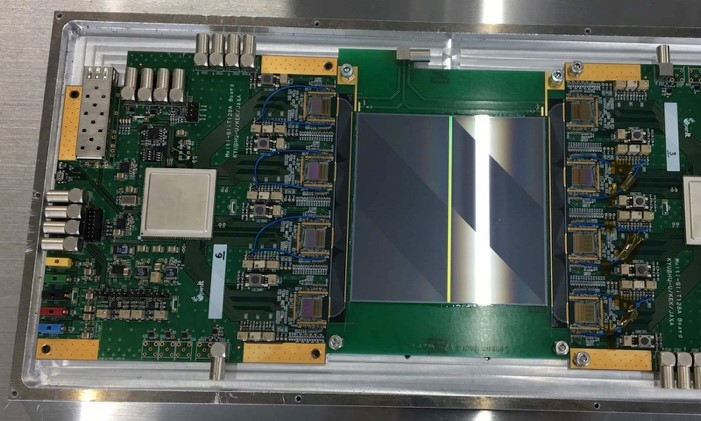
\includegraphics[width=0.7\textwidth, bb=0 0 229 138]
                 {./Fig/MuHFS-IntegratedSiliconStripDetector.jpg}
\caption{\label{fig:MuSEUM-IntegratedSiliconStripDetector}
Integrated silicon strip detector.  The sensor is directly
connected on both sides to an analog/digital combined type
integrated circuit for readout and signal processing through
four ASIC-ASDs (Slit128A) controlled by a FPGA.}
\end{figure}

High-field measurements will be performed with a superconducting
solenoid magnet that was recycled from an old MRI magnet designed
for high homogeneous magnetic field.The choice of a longer cavity
to allow measurement at lower Kr gas density imposes strict
requirements on the magnet.  Indeed, the systematic uncertainty
on the magnetic field was the second largest uncertainty in
the previous experiment at LAMPF \cite{Liu:1999iz}.  
The muonium HFS frequency
$\Delta \nu_{\text{HFS}} (=\nu_{12}+\nu_{34})$ is in principle
independent of the magnetic field.  However, $\mu_\mu/\mu_p$
($=\nu_{34}- \nu_{12}$) is dependent on the magnetic field, 
and its inhomogeneity relates largely to the systematic
uncertainty.  But since both $\nu_{12}$ and $\nu_{34}$ are
measured separately, a precise calibration is still required
in both cases.  The present requirements for the magnetic
field are a homogeneity of $<1$ ppm with absolute calibration
in a spheroidal volume of $\phi 200$ mm $\times$ 300 mm
(muon stopping region), a field stability of 0.1 ppm/h,
and an absolute calibration at 10 ppb level.  Improvement
of the homogeneity of the MRI magnet and development of NMR
probes for absolute magnetic field calibration is steadily
progressing.


Commissioning test of the MRI magnet was performed.After several
iterative shimming processes, a field homogeneity within 0.8
ppm peak-to-peak in the muon stopping spheroid was reached.
The long-term stability was measured at 3 ppb/hour over a 10
days period.  The helium evaporation rate was 3 L/day.  All
this fulfills our design values.

For the precise magnetic field monitoring, a continuous wave
NMR (CW-NMR) system with a RF pickup coil is being developed
for both $g-2$/EDM and MuSEUM experiments at J-PARC.  A field
mapping probe with 24 RF pickup coils is being constructed
to scan the muon stopping spheroid inside the MRI magnet.
Also, a cross calibration test is in progress at Argonne
National Laboratory with the pulse-NMR probe used at the
FermiLab muon storage ring experiment \cite{Bennett:2006fi}.
The magnetic field is measured at the same position by both
probes.  The development of the CW-NMR probe is reported in
details in \cite{T.Tanaka-etal-PSAS2018}.  Preliminary
measurements showed that a resolution of 18 ppb could be
reached \cite{Sasaki-etal-IEEE}.  Recently, even better
resolution was obtained, but the analysis is still in progress
and the results will be published elsewhere.


Commissioning test experiments at zero field are being performed
since February 2016 at the D2 experimental area (D-Line) of
the MUSE facility.  These engineering runs are crucial to test
the different aspects of the apparatus and grasp possible
problems to be overcome before the start of the high-field
measurements.  Zero-field measurements are also important
because of different systematics from the magnetic field
(negligible at zero field).  Figure \ref{fig:MuSEUM-ZeroFieldExp-setup}
shows the apparatus during one of the engineering runs.  
The residual magnetic field is suppressed below 100 nT
by a magnetic shield made of three layers of 1.5-mm thick
permalloy that enclose completely the gas chamber and RF cavity.

\begin{figure}
 \centering
\begin{overpic}[width=0.7\textwidth,bb=0 0 701 525]
                 {./Fig/image017.jpg}
\put(0,-3.5){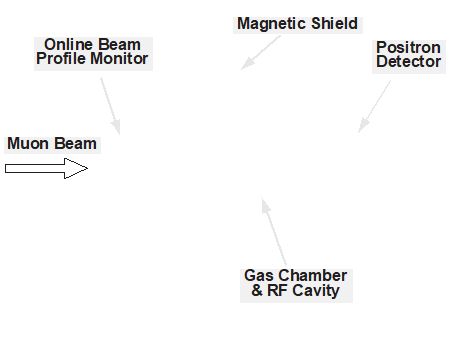
\includegraphics[width=0.75\textwidth, bb=0 0 227 170]
{./Fig/MuHFS-MuSEUM-ZeroFieldExp-setup.png}}
\end{overpic}
\caption{\label{fig:MuSEUM-ZeroFieldExp-setup}
Experimental setup for zero-field measurements at area D2 of MUSE D-Line.
}
\end{figure}


Since the first resonance peak was observed in June 2016,
systematic uncertainties due to gas pressure and impurity,
RF power stability and muon beam profile distribution were
studied.  As we improve the statistics, the systematic uncertainty
becomes more severe and needs to be carefully considered.
It should be noted that our understanding of the systematical
error in an experiment is limited by the time spent on the
measurements, and that longer the measurement time, the
lower the systematic uncertainty.


Figure \ref{fig:MuSEUM-MuSEUM-lineshape} shows a typical
resonance lineshape of the muonium HFS transition as a
function of the applied RF frequency detuned from 4463.3 MHz
measured in March 2018 (scintillation detector data).
The time integral method is used by measuring alternatively
RF ON and OFF at different detuning frequencies and taking
the difference, i.e., 
$(N_{\text{ON}}-N_{\text{OFF}})/N_{\text{OFF}}$.  
The blue line shows a preliminary Lorentzian fitting result.
   

\begin{figure}[th]
 \centering
 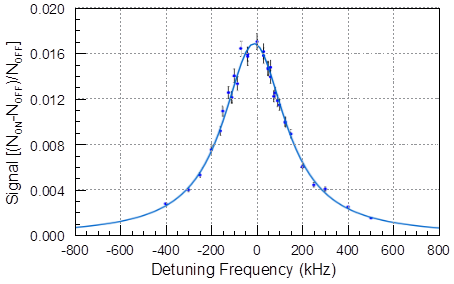
\includegraphics[width=0.7\textwidth, bb=0 0 227 142]
                 {./Fig/MuHFS-MuSEUM-lineshape.png}
\caption{\label{fig:MuSEUM-MuSEUM-lineshape}
Typical muonium HFS transition resonance lineshape as a
function of the applied RF frequency detuned from 4463.3 MHz.
The blue line shows a preliminary Lorentzian fitting result.
The data analysis is in progress.
}
\end{figure}


New precise muonium HFS measurements are important for further
QED testing and new fundamental physics experiments.  Improving
the overall accuracy, estimating and understanding systematic
uncertainties are essential in reaching that goal.  Measurements
at zero field are yielding their first results at MUSE D-Line.
Preparation for the high-field measurements at H-Line are
steadily progressing.  At present, it is unclear when the
new H-Line will be operational, but we are aiming at a first
test experiment at high field sometime in 2019-2020.




\section{Summary}

\section*{Acknowledgments}
The authors would like to thank the KEK and the J-PARC muon section staffs for their strong support.
This work is supported by JSPS KAKENHI Grants No.~JP19740158, No.~JP23108001, No.~JP23740216, No.~JP25800164, No.~JP26287053, No.~JP26287055, No.~ JP15H03666, No.~JP15H05742, No.~JP16H03987, No.~JP16J07784, No.~JP16K13810, No.~JP16K05323, No.~JP17H01133, No.~JP17H02904, No.~JP17K05466, No.~JP17K18784, No.~JP18H01239 and No.~JP18H03707. 
This work is also supported by the Korean National Research Foundation Grants No.~NRF- 2015H1A2A1030275, No.~NRF-2015K2A2A4000092, and No. NRF-2017R1A2B3007018; 
the Russian Foundation for Basic Research Grant No.~RFBR 17-52-50064 and No.~RNF 17-12-01036 which are a part of the Japan-Russia Research Cooperative Program;
the U.S.-Japan Science and Technology Cooperation Program in High Energy Physics;
and the Discovery Grants Program of the Natural Sciences and Engineering Research Council of Canada.


%\bibliographystyle{frontiersinSCNS_ENG_HUMS} % for Science, Engineering and Humanities and Social Sciences articles, for Humanities and Social Sciences articles please include page numbers in the in-text citations
\bibliographystyle{frontiersinHLTH&FPHY} % for Health, Physics and Mathematics articles
%\bibliography{test}
%\bibitem{proposal} E34 proposal, 2010 (unpublished).
\bibitem{CDR} E34 conceptual design report, 2011 (unpublished).
\bibitem{E821} G. W. Bennett {\it et al.}, Phys. Rev. D {\bf 73}, 072003 (2006).
\bibitem{FNAL_E989_TDR} J.~Grange {\it et al.}, "Muon ($g-2$) Technical Design Report'', arXiv:1501.06858 (2015).
\bibitem{E821-EDM} G. W.~Bennett {\it et al.}, Phys. Rev. D {\bf 80}, 052008 (2009).

\bibliography{ref_g-2edm}

%%% Make sure to upload the bib file along with the tex file and PDF
%%% Please see the test.bib file for some examples of references

%%% If you are submitting a figure with subfigures please combine these into one image file with part labels integrated.
%%% If you don't add the figures in the LaTeX files, please upload them when submitting the article.
%%% Frontiers will add the figures at the end of the provisional pdf automatically
%%% The use of LaTeX coding to draw Diagrams/Figures/Structures should be avoided. They should be external callouts including graphics.

\end{document}
